\documentclass[12pt,a4paper]{article}
%\usepackage[T1]{fontenc}
%\usepackage[utf8]{inputenc}
\usepackage[spanish]{babel}
%%INICIO DE TIPO DE LETRA 
\usepackage{newtxtext,newtxmath}
%TIPO DE LETRA FIN
\usepackage{tocloft}


\setlength{\textwidth}{16cm}
\usepackage{amsmath, amsfonts}
\usepackage{graphicx}
\usepackage{alltt}
\usepackage{hyperref}
%\usepackage{lmodern}
\usepackage{hyperref}
\usepackage{tikz}
\usepackage{gensymb}
\usepackage[titletoc]{appendix}
\usepackage{tabto}
\usepackage{float}
\usepackage{dashrule}
\usepackage{subfig}
\usetikzlibrary{intersections,calc,positioning,shapes.geometric,arrows.meta,chains,babel}
\usepackage{pdfpages}
\usepackage{listings}
\usepackage{color}
\usepackage{caption}
\usepackage{newclude}
\usepackage{tabularx}

\usepackage{fancyhdr}
%\usepackage{geometry}
\usepackage[
  a4paper,
  left=3.0cm,
  right=2.5cm,
  top=2.5cm,
  bottom=2.5cm
]{geometry}
\usepackage{pdfpages}
\usepackage{numprint}
\usepackage{multirow}
\usepackage{arydshln}
\usepackage{titlesec}
\usepackage{chngcntr}
\usepackage{cleveref}
%%%%%%%%%%%%%%%%%%%%%%%%%
\usepackage{ragged2e}
%%%% titulos y subtitulos mismo tamaño %%%%
\usepackage[modulo]{lineno}
% ==== NUMERACIÓN DE LÍNEAS DESDE EL ÍNDICE ====

% Fuente y posición de los números
\renewcommand\linenumberfont{\normalfont\bfseries\scriptsize}
\setlength\linenumbersep{10pt}

% Mantener numeración al usar clearpage o input
\makeatletter
\let\old@clearpage\clearpage
\renewcommand{\clearpage}{%
  \ifLineNumbers
    \old@clearpage
    \linenumbers
  \else
    \old@clearpage
  \fi
}
\makeatother

\usepackage{xpatch}
\usepackage{lipsum}
%numeracion parte superior
\usepackage{lastpage}
\pagestyle{fancy}
\usepackage{csquotes}

\usepackage[style=iso-authoryear,backend=biber]{biblatex}
\addbibresource{OLD_BIBLIO.bib}
%%mayuscula los autores
\AtBeginBibliography{%
  \renewcommand*{\mkbibnamefamily}[1]{\MakeUppercase{#1}}%
}

% --- Color azul en TODAS las citas ---
\usepackage{xcolor}

% Paréntesis en azul
\let\oldmkbibparens\mkbibparens
\renewcommand*{\mkbibparens}[1]{\textcolor{blue}{\oldmkbibparens{#1}}}

\usepackage{xcolor}
\AtEveryCitekey{\color{blue}}

\usepackage{enumerate}
\usepackage{enumitem}

\usepackage{pgfplots}
\usepackage{bchart}
\pgfplotsset{compat=1.18}

\newcommand{\aref}[1]{\hyperref[#1]{Appendix~\ref{#1}}}
\setlength\dashlinedash{0.5pt}
\setlength\dashlinegap{3pt}

% Estilo ISO 690 para tablas
\DeclareCaptionLabelSeparator{iso690sep}{\space—\space}
\captionsetup[table]{
  labelfont=bf,
  labelsep=iso690sep,
  textfont=bf,
  justification=raggedright,
  singlelinecheck=false,
  name=Tabla,
  font=normalfont,
  skip=1ex
}

% Estilo ISO 690 para figuras
\captionsetup[figure]{
  labelfont=bf,
  labelsep=iso690sep,
  textfont=bf,
  justification=raggedright,
  singlelinecheck=false,
  name=Figura,
  font=normalfont,
  skip=1ex
}
\addto\captionsspanish{\renewcommand{\tablename}{Tabla}}
\addto\captionsspanish{\renewcommand{\figurename}{Figura}}

%sub nivel 4
\titleformat{\paragraph}[hang]{\normalfont\fontsize{13pt}{12pt}\bfseries}{\theparagraph}{1em}{}
\titlespacing*{\paragraph}{0pt}{1.5ex plus 0.5ex minus .2ex}{1em}
\setcounter{secnumdepth}{4}

% Configurar líneas gruesas
\setlength{\arrayrulewidth}{0.75pt}
\newcommand{\thickhline}{\Xhline{1.2pt}}

\usepackage{caption}
\DeclareCaptionLabelSeparator{emdash}{\textemdash\ }
\captionsetup[table]{labelformat=default, labelsep=emdash, justification=raggedright}
\captionsetup[figure]{labelformat=default, labelsep=emdash, justification=raggedright}

\makeatletter
\def\thickhline{%
  \noalign{\ifnum0=`}\fi
    \hrule \@height 2pt
  \futurelet\reserved@a\@xhline}
\makeatother

\renewcommand{\cftsecleader}{\cftdotfill{\cftdotsep}}

% ===== Listas alineadas con párrafo =====
\setlist[itemize]{label=\textbullet}

% ======= FORMATO TÍTULOS Y ALINEACIÓN =======

% --- Section ---
\newlength{\numwidthsec}
\setlength{\numwidthsec}{3em}
\titleformat{\section}[hang]
  {\normalfont\fontsize{12pt}{12pt}\bfseries}
  {\makebox[\numwidthsec][l]{\thesection}}
  {0pt}{}

% --- Subsection ---
\newlength{\numwidthsub}
\setlength{\numwidthsub}{3em}
\titleformat{\subsection}[hang]
  {\normalfont\fontsize{12pt}{12pt}\bfseries}
  {\makebox[\numwidthsub][l]{\thesubsection}}
  {0pt}{}

% --- Subsubsection ---
\titleformat{\subsubsection}[hang]
  {\normalfont\fontsize{12pt}{12pt}\bfseries}
  {\thesubsubsection}{0.0em}{}

% --- Sangría general ---
\setlength{\parindent}{0pt}

% --- Reglas de sangría según nivel ---
\pretocmd{\section}{\setlength{\leftskip}{2.5em}}{}{}
\pretocmd{\subsection}{\setlength{\leftskip}{4.5em}}{}{}
\pretocmd{\subsubsection}{\setlength{\leftskip}{7.5em}}{}{}
\pretocmd{\paragraph}{\setlength{\leftskip}{11.5em}}{}{}

\setlength{\numwidthsec}{3em}
\titleformat{\section}[hang]
  {\normalfont\fontsize{12pt}{12pt}\bfseries}
  {\makebox[\numwidthsec][l]{\thesection}}
  {0pt}{}

\setlength{\numwidthsub}{3em}
\titleformat{\subsection}[hang]
  {\normalfont\fontsize{12pt}{12pt}\bfseries}
  {\makebox[\numwidthsub][l]{\thesubsection}}
  {0pt}{}

\titleformat{\subsubsection}[block]
  {\normalfont\fontsize{12pt}{12pt}\bfseries}
  {\thesubsubsection}{1.0em}{}{}

% --- Espaciado títulos ---
\titlespacing*{\section}{0.0em}{1.5em}{1pt}
\titlespacing*{\subsection}{1.5em}{1.5em}{0pt}
\titlespacing*{\subsubsection}{4.5em}{1.5em}{0pt}
\titlespacing*{\paragraph}{7.5em}{1.5em}{0pt}

% --- Sangría general ---
\setlength{\parindent}{1.5pt}

% ===== Listas =====
\setlist[itemize,1]{label=\textbullet, labelsep=1em}
\setlist[enumerate,1]{label=\arabic*., labelsep=1em}

\pretocmd{\section}{\setlist[itemize,1]{left=0.5em,labelsep=1em}\setlist[enumerate,1]{left=0.5em,labelsep=1em}}{}{}
\pretocmd{\subsection}{\setlist[itemize,1]{left=4.5em,labelsep=1em}\setlist[enumerate,1]{left=4.5em,labelsep=1em}}{}{}
\pretocmd{\subsubsection}{\setlist[itemize,1]{left=7.3em,labelsep=1em}\setlist[enumerate,1]{left=7.3em,labelsep=1em}}{}{}
\pretocmd{\paragraph}{\setlist[itemize,1]{left=10.5em,labelsep=1em}\setlist[enumerate,1]{left=10.5em,labelsep=1em}}{}{}

%%numeracion
\usepackage{fancyhdr}
\usepackage{lastpage}

% --- Estilo general de páginas ---
\pagestyle{fancy}
\fancyhf{}
\fancyhead[R]{%
\textbf{- \thepage}\ de\ \textbf{\pageref{LastPage} -}%
}
\fancyfoot{}
\renewcommand{\headrulewidth}{0pt}

%%%AJUSTAR LOS TEXTOS
\makeatletter
\def\@afterheading{%
  \@nobreaktrue
  \everypar{%
    \@nobreakfalse
    \clubpenalty\@M
    \widowpenalty\@M
    \everypar{}%
    \setlength{\parindent}{0em}%
  }%
}
\makeatother

%%INTERLINEADO
\usepackage{etoolbox}
\usepackage{setspace}
\usepackage{capt-of}

%%%%%%%%%%
% --- Nuevo entorno alineado ---
\newenvironment{alignedfigure}
  {\par\hspace*{3em}\begin{minipage}{0.95\linewidth}}
  {\end{minipage}\par}

%%NUMERACION DE LAS LINEAS
\renewcommand\linenumberfont{\normalfont\fontsize{12}{12}\selectfont}

\makeatletter
\newcommand{\blanklines}[1]{%
  \par
  \begingroup
  \@tempcnta=0
  \loop
    \advance\@tempcnta by 1
    \noindent\null\par
    \ifnum\@tempcnta<#1
  \repeat
  \endgroup
}
\makeatother

\newcommand{\parnumerado}{\noindent\null\par}
\setlength\linenumbersep{1em}
\modulolinenumbers[1]

\setlist[itemize]{label=\textbullet}

%%ALINEAR FIGURAS Y TABLAS DENTRO DE LA SECCION
\usepackage{changepage}
\newenvironment{levelaligned}
{
  \begin{adjustwidth}{\leftskip}{0pt}
  \begin{minipage}{0.95\linewidth}
}
{
  \end{minipage}
  \end{adjustwidth}
}

% ===============================
% FORMATO DEL ÍNDICE (TOC)
% ===============================

% --- Quitar negrita en secciones del TOC ---
\renewcommand{\cftsecfont}{\normalfont}
\renewcommand{\cftsecpagefont}{\normalfont}

% --- Sangrías: títulos sin número al margen, numerados con sangría ---
\renewcommand{\cftsecindent}{0pt}
\renewcommand{\cftsubsecindent}{1.2em}
\renewcommand{\cftsubsubsecindent}{1.2em}

% --- Espacio reservado para los números ---
\setlength{\cftsecnumwidth}{2.2em}
\setlength{\cftsubsecnumwidth}{3.0em}
\setlength{\cftsubsubsecnumwidth}{3.0em}

% --- Líneas punteadas en todos los niveles ---
\renewcommand{\cftsecleader}{\cftdotfill{\cftdotsep}}
\renewcommand{\cftsubsecleader}{\cftdotfill{\cftdotsep}}
\renewcommand{\cftsubsubsecleader}{\cftdotfill{\cftdotsep}}

% --- Sin espacio extra entre entradas ---
\setlength{\cftbeforesecskip}{0pt}
\setlength{\cftbeforesubsecskip}{0pt}
\setlength{\cftbeforesubsubsecskip}{0pt}

% ===============================
% Formato Índice de Tablas — espaciado simétrico alrededor del guión
% ===============================
\renewcommand{\cfttabpresnum}{\textbf{Tabla~}}
\renewcommand{\cfttabaftersnum}{\textbf{~\textemdash~}}
\newlength{\mylenT}
\settowidth{\mylenT}{\cfttabpresnum 9\cfttabaftersnum}
\setlength{\cfttabnumwidth}{\mylenT}

% ===============================
% Formato Índice de Figuras — espaciado simétrico alrededor del guión
% ===============================
\renewcommand{\cftfigpresnum}{\textbf{Figura~}}
\renewcommand{\cftfigaftersnum}{\textbf{~\textemdash~}}
\newlength{\mylenF}
\settowidth{\mylenF}{\cftfigpresnum 9\cftfigaftersnum}
\setlength{\cftfignumwidth}{\mylenF}

% ===============================
% Títulos de índices centrados
% ===============================
\addto\captionsspanish{%
  \renewcommand{\listtablename}{\hfill ÍNDICE DE TABLAS\hfill}%
  \renewcommand{\tablename}{Tabla}%
  \renewcommand{\listfigurename}{\hfill ÍNDICE DE FIGURAS\hfill}%
  \renewcommand{\figurename}{Figura}%
}

\newcommand{\DisableFancyAll}{%
  \fancyhf{}%
  \fancyhead{}%
  \fancyfoot{}%
  \renewcommand{\headrulewidth}{0pt}%
  \renewcommand{\footrulewidth}{0pt}%
}

%%ecuacion por capitulo
\usepackage{chngcntr}
\counterwithin{equation}{section}
\renewcommand{\theequation}{\thesection.\arabic{equation}}

%%%rotar la tabla
\usepackage{rotating}
\usepackage{pifont}
\usepackage{pdflscape}
\usepackage{makecell}
\usepackage{afterpage}

%%codigo python
\usepackage{listings}
\usepackage{xcolor}

\lstset{
  language=Python,
  basicstyle=\ttfamily\scriptsize,
  keywordstyle=\color{blue},
  commentstyle=\color{gray},
  stringstyle=\color{red},
  numbers=left,
  numberstyle=\tiny,
  stepnumber=1,
  numbersep=3pt,
  frame=single,
  breaklines=true,
  captionpos=b
}
\lstset{
  extendedchars=true,
  inputencoding=utf8,
  literate=
    {á}{{\'a}}1 {é}{{\'e}}1 {í}{{\'i}}1 {ó}{{\'o}}1 {ú}{{\'u}}1
    {Á}{{\'A}}1 {É}{{\'E}}1 {Í}{{\'I}}1 {Ó}{{\'O}}1 {Ú}{{\'U}}1
    {ñ}{{\~n}}1 {Ñ}{{\~N}}1
    {Δ}{{$\Delta$}}1
    {β}{{$\beta$}}1
    {γ}{{$\gamma$}}1
    {ζ}{{$\zeta$}}1
}

\onehalfspacing

\begin{document}
% --- Portada ---
\newpage
\thispagestyle{empty}
\linenumbers
\noindent
\title{Tesis Sistemas}
\begin{center}
\vspace{1mm}
{\fontsize{12pt}{14pt}\textbf{UNIVERSIDAD NACIONAL MICAELA BASTIDAS DE APURÍMAC}}\\
\vspace{2mm}
{\fontsize{12pt}{14pt}\textbf{FACULTAD DE INGENIERÍA}}\\
\blanklines{2} % crea 2 líneas numeradas en blanco
{\fontsize{12pt}{14pt}ESCUELA ACADÉMICO PROFESIONAL DE INGENIERÍA INFORMATICA Y SISTEMAS}\\[4mm]

\includegraphics[keepaspectratio,scale=0.85]{Logo_unamba.png} \\
\blanklines{2} % crea 2 líneas numeradas en blanco
{\fontsize{12pt}{12pt}\selectfont Proyecto de Tesis}\\[-0.1cm]
\blanklines{1}
{\fontsize{12pt}{14pt}\selectfont
Ecosistema Inteligente con Visión Artificial y LLM para mejorar el
rendimiento académico en la UNAMBA, 2026 }
\blanklines{1} % linea en blanco
Presentado por: \\
\blanklines{2} % crea 2 líneas numeradas en blanco
Clinio Omar Rayme Huacho \\
\blanklines{1}  % linea en blanco
Para optar el título de Ingeniero Informatico y Sistemas \\
\blanklines{4} % crea 4 líneas numeradas en blanco
{\fontsize{12pt}{14pt} Abancay, Perú}\\[0.3cm]
{\fontsize{12pt}{14pt} 2026}
\end{center}


% \clearpage
\thispagestyle{empty}
\begin{center}
\vspace{5mm}
{\fontsize{12pt}{14pt}\textbf{UNIVERSIDAD NACIONAL MICAELA BASTIDAS DE APURÍMAC}}\\[1mm]
{\fontsize{12pt}{14pt}\textbf{FACULTAD DE INGENIERÍA}}\\[1mm]
{\fontsize{12pt}{14pt}ESCUELA PROFESIONAL DE INGENIERÍA INFORMATICA Y SISTEMAS}\\
\blanklines{2} % CREA ESPACION EN BLANCO

\includegraphics[keepaspectratio,scale=0.6]{logo.jpg}\\
\blanklines{2} % CREA ESPACIO EN BLANCO
{TESIS}
\blanklines{1} %espacio en blanco
\fontsize{12pt}{10pt}
\textbf{Ecosistema Inteligente con Visión Artificial y LLM para mejorar el
Rendimiento Académico en la UNAMBA, 2026}
\end{center}
\blanklines{1} %espacio en blanco
\fontsize{12pt}{14pt}
\hspace{0.5cm} Presentado por \textbf{Clinio Omar Rayme Huacho}, para optar el título de Ingeniero Informatico y Sistemas 
\blanklines{1} %espacio en blanco
Sustentado y aprobado \hspace{0.2cm}\dotfill\hspace{0.3cm}
(fecha de sustentación)
\hspace{0.2cm}\dotfill\hspace{0.3cm}
ante el jurado evaluador:

\blanklines{1} %espacio en blanco

\nolinenumbers   % desactiva numeración de líneas

\noindent
\fontsize{12pt}{14pt}\selectfont

\begin{tabular}{r p{8cm}}
\textbf{Presidente:} & \underline{\hspace{8cm}} \\[-0.2cm]
& \hspace{1cm}\footnotesize \textit{Grado. Nombres y apellidos} \\[0.7cm]

\textbf{Primer miembro:} & \underline{\hspace{8cm}} \\[-0.2cm]
& \hspace{1cm}\footnotesize \textit{Grado. Nombres y apellidos} \\[0.7cm]

\textbf{Segundo miembro:} & \underline{\hspace{8cm}} \\[-0.2cm]
& \hspace{1cm}\footnotesize \textit{Grado. Nombres y apellidos} \\[0.7cm]

\textbf{Asesor:} & \underline{\hspace{8cm}} \\[-0.2cm]
& \hspace{1cm}\footnotesize \textit{M.Sc. Yhon Fuentes Huaman} \\[0.5cm]
\end{tabular}

\linenumbers   % vuelve a activar numeración si la usas después




% \nolinenumbers

% \newpage
% \thispagestyle{empty}
% \input{Constancia_originalidad}

% \newpage
% \thispagestyle{empty}
% \vfill

\begin{flushright}
\textbf{\underline{Agradecimiento}}
\end{flushright}

\vspace{0.5cm}

\begin{flushright}
\begin{minipage}{0.7\textwidth}
\itshape
\justify
A la Universidad Nacional Micaela Bastidas de Apurímac y de manera especial a la Escuela Académico Profesional de Ingeniería de Informática y Sistemas, por haberme brindado el espacio institucional y las herramientas necesarias para mi formación profesional y científica.

A nuestros asesores y docentes de la facultad, cuyos rigurosos comentarios, correcciones y constante exigencia metodológica permitieron reorientar el enfoque de esta investigación hacia un impacto real y medible en el aprendizaje estudiantil.

A los compañeros de equipo y de ruta académica, por el soporte técnico incondicional, las largas noches de debate arquitectónico y el esfuerzo compartido en la construcción de este proyecto; este logro es también el reflejo de nuestra dedicación colectiva.

Finalmente, a cada uno de los estudiantes de nuestra casa de estudios que participaron activamente en las pruebas experimentales, cuya retroalimentación e interacciones semánticas dieron vida y validaron el propósito de este ecosistema digital.
\end{minipage}
\end{flushright}

% \newpage
% \thispagestyle{empty}
% \vfill

\begin{flushright}
\textbf{\underline{Dedicatoria}}
\end{flushright}

\vspace{0.5cm}

\begin{flushright}
\begin{minipage}{0.7\textwidth}
\itshape
\justify
A mis padres, por su amor incondicional, su paciencia infinita y por ser el pilar fundamental que sostuvo cada uno de mis pasos a lo largo de este trayecto académico y personal. 

A mi familia, por sus palabras de aliento en los momentos de mayor exigencia y por creer firmemente en mi capacidad para alcanzar mis metas.

Y a todas las personas que, de manera silenciosa pero constante, compartieron sus conocimientos, su tiempo y su apoyo, motivándome a culminar con éxito esta importante etapa de formación profesional.
\end{minipage}
\end{flushright}
% \linenumbers

\newpage

% --- INDICE GENERAL ---
\clearpage
\pagenumbering{gobble}
\pagestyle{empty}
\blanklines{4}

\renewcommand{\contentsname}{%
  \begin{center}\MakeUppercase{\fontsize{12pt}{12pt}\selectfont ÍNDICE}\end{center}%
}

\addtocontents{toc}{\protect\flushright{\fontsize{12pt}{12pt}\selectfont Pag.}\par}

\begingroup
\makeatletter
\renewcommand{\numberline}[1]{#1\quad}
\makeatother
\tableofcontents
\endgroup
\clearpage

% --- INDICE DE TABLAS---
\clearpage
\DisableFancyAll
\thispagestyle{empty}
\blanklines{4}
\listoftables

% --- INDICE DE FIGURAS ---
\newpage
\clearpage
\thispagestyle{empty}
\blanklines{4}
\listoffigures

\clearpage
\pagestyle{fancy}
\fancyhf{}
\fancyhead[R]{%
\textbf{- \thepage}\ de\ \textbf{\pageref{LastPage} -}%
}
\renewcommand{\headrulewidth}{0pt}

\newpage
\clearpage
\pagenumbering{arabic}
\blanklines{4}
\begin{center}
\textbf{INTRODUCCIÓN}
\end{center}
\addcontentsline{toc}{section}{INTRODUCCIÓN}


La adopción de la Inteligencia Artificial Generativa ha impulsado una transformación sin precedentes en la educación superior, redefiniendo las metodologías de enseñanza y la asimilación del conocimiento \parencite{Vieriu2025}. En este escenario, la gestión de apuntes universitarios ha experimentado una evolución acelerada, migrando desde los métodos manuscritos tradicionales hacia formatos digitales dinámicos e interactivos. Esta transición tecnológica busca optimizar la captura, organización y recuperación de la información académica. Según \textcite{Kreijkes2026}, la integración de Modelos de Lenguaje Grande (LLMs) presenta oportunidades excepcionales para facilitar la comprensión lectora y reducir la carga cognitiva inicial de los estudiantes. Sin embargo, el volumen exponencial de datos técnicos y científicos en disciplinas de ingeniería exige herramientas que trasciendan el simple almacenamiento, demandando ecosistemas capaces de procesar y enlazar semánticamente el contenido educativo.\\

A pesar de estos avances tecnológicos, la digitalización educativa contemporánea enfrenta desafíos algorítmicos y pedagógicos severos. Los estudiantes de ingeniería padecen de una constante sobrecarga cognitiva al intentar integrar múltiples fuentes de información no estructurada. La adopción pasiva de plataformas de IA genéricas agrava este panorama, induciendo una dependencia tecnológica que inhibe el análisis crítico y la apropiación del conocimiento \parencite{Vieriu2025}. A nivel técnico, los LLMs estándar adolecen de un problema crítico de "alucinaciones"; dado que carecen de mecanismos intrínsecos para verificar la veracidad de los hechos, frecuentemente generan información plausible pero fácticamente incorrecta \parencite{Chen2023}. Adicionalmente, la digitalización de apuntes científicos enfrenta la barrera de la notación matemática, donde los sistemas tradicionales fracasan al procesar estructuras espaciales complejas \parencite{AlvarezPerez2026}. Finalmente, las herramientas actuales promueven un consumo individualista y fragmentado de la información, careciendo de la infraestructura lógica para establecer vínculos semánticos que fomenten una colaboración auténtica entre pares \parencite{Jiang2025}.\\

Para mitigar estas brechas tecnológicas y metodológicas, la presente investigación propone formalmente el desarrollo de SynapTome, un ecosistema digital inteligente y colaborativo fundamentado en los principios de la Arquitectura Limpia (Clean Architecture). La infraestructura del sistema orquesta tecnologías de vanguardia para transformar la gestión del aprendizaje: en el núcleo de procesamiento de lenguaje natural, se implementa una arquitectura de Generación Aumentada por Recuperación (RAG) que restringe la inferencia de la IA a un corpus documental validado, garantizando precisión factual y eliminando las alucinaciones \parencite{Ning2025}. Para abordar el reto de la digitalización científica, se integra un pipeline de visión por computadora basado en el modelo Transformer TrOCR, el cual permite la transcripción estructurada de apuntes manuscritos y fórmulas matemáticas al formato LaTeX \parencite{KardanMoghaddam2025}. El elemento diferenciador de SynapTome radica en su motor de base de datos relacional modelado mediante Grafos de Conocimiento en PostgreSQL. Estos grafos indexan topológicamente los bloques de estudio, descubriendo relaciones transversales entre múltiples usuarios para catalizar una verdadera "Inteligencia Colectiva" \parencite{Obionwu2022}. Todo el ecosistema opera con una sincronización concurrente a través de SignalR y C\#, con una interfaz reactiva desarrollada en Next.js.\\

El presente trabajo de investigación se estructura en cinco capítulos secuenciales que detallan el ciclo de vida del proyecto: el Capítulo I expone el planteamiento del problema, su justificación y el contexto universitario del caso de estudio; el Capítulo II detalla los objetivos generales y específicos, así como las hipótesis de investigación y la operacionalización de variables; el Capítulo III desarrolla el marco teórico referencial, profundizando en los fundamentos de las arquitecturas RAG, TrOCR y la teoría subyacente de los Grafos de Conocimiento; el Capítulo IV describe el diseño metodológico, definiendo el enfoque experimental, las métricas de evaluación técnica y los instrumentos de usabilidad; finalmente, el Capítulo V presenta la arquitectura de software implementada, el análisis de los resultados obtenidos durante el despliegue del sistema y las conclusiones finales derivadas del proyecto.

\clearpage
\blanklines{4}
\setcounter{section}{1}
\setcounter{subsection}{0}
\begin{center}
\textbf{DATOS GENERALES}
\end{center}
\addcontentsline{toc}{section}{\textbf{DATOS GENERALES}}
\addcontentsline{toc}{subsection}{\protect\numberline{\textbf{a)}}\textbf{Título del proyecto:}}
\addcontentsline{toc}{subsection}{\protect\numberline{\textbf{b)}}\textbf{Ejecutor/ejecutores:}}
\addcontentsline{toc}{subsection}{\protect\numberline{\textbf{c)}}\textbf{Coasesor (si hubiese):}}
\addcontentsline{toc}{subsection}{\protect\numberline{\textbf{d)}}\textbf{Línea de investigación:}}
\begin{enumerate}[label=\alph*)]
    \item \textbf{Título del proyecto:}

    Ecosistema Inteligente con Visión Artificial y LLM para mejorar el Aprendizaje Colaborativo en la UNAMBA, 2026\\
	
    \item \textbf{Ejecutor:}
    \begin{itemize}[label=\textbullet, leftmargin=0.55cm]
        \item Clinio Omar Rayme Huacho \\
    \end{itemize} % <-- SIN "\\" AQUÍ
    
    \item \textbf{Asesor:}
    \begin{itemize}[label=\textbullet, leftmargin=0.55cm]
        \item M.Sc. Yhon Fuentes Huaman \\
    \end{itemize} % <-- SIN "\\" AQUÍ
    
    \item \textbf{Línea de investigación:}
    \begin{itemize}[label=\textbullet, leftmargin=0.55cm]
        \item Ingeniería de software e innovación tecnológica \\
    \end{itemize} % <-- SIN "\\" AQUÍ
   
\end{enumerate}

% --- CAPÍTULO I ---
\clearpage
\blanklines{4}
\setcounter{section}{1}
\setcounter{subsection}{0}
\begin{center}
\textbf{CAPÍTULO I}\\
\textbf{PLANTEAMIENTO DEL PROBLEMA}
\end{center}
\input{Cap1_planteamientoProblema}

% --- CAPÍTULO II ---
\clearpage
\blanklines{4}
\setcounter{section}{2}
\setcounter{subsection}{0}
\begin{center}
\textbf{CAPÍTULO II} \\
 \textbf{OBJETIVOS E HIPÓTESIS}
\end{center}
\addcontentsline{toc}{section}{\textbf{CAPÍTULO II}}
\addcontentsline{toc}{section}{\textbf{OBJETIVOS E HIPÓTESIS}}

\subsection{Objetivos de la investigación}

%====================================================
\subsubsection{Objetivo general}
%====================================================
Reducir la sobrecarga de apuntes y la fatiga mental, y optimizar el rendimiento académico de los estudiantes universitarios de la UNAMBA al implementar y evaluar una aplicación web basada en un entorno de aprendizaje interconectado y automatizado.

%====================================================
\subsubsection{Objetivos específicos}
%====================================================
\begin{itemize}

\item 
Reducir el tiempo dedicado a la consolidación de apuntes manuscritos y aumentar la tasa de preservación de información técnica mediante el uso de la aplicación web con un módulo de transcripción automatizada (TrOCR).

\item
Reducir la tasa de errores conceptuales en el material de repaso de los estudiantes al condicionar las respuestas de la aplicación web mediante un middleware RAG acoplado a un LLM en comparación con el uso de herramientas de entorno abierto.

\item
Disminuir el nivel de sobrecarga cognitiva y la fatiga mental, y optimizar el rendimiento académico de los alumnos al implementar en la aplicación web un motor relacional de grafos de conocimiento con evaluaciones dinámicas automatizadas.

\end{itemize}
\subsection{Hipótesis de la investigación}

%====================================================
\subsubsection{Hipótesis general}
%====================================================
La transición desde esquemas tradicionales de gestión de estudio aislados hacia el uso adaptativo del ecosistema inteligente optimiza significativamente el rendimiento académico y reduce la sobrecarga cognitiva en los estudiantes universitarios, en la UNAMBA, 2026.

%====================================================
\subsubsection{Hipótesis específicas}
%====================================================
\begin{itemize}

\item
La migración de los estudiantes hacia un flujo de digitalización automatizado mediante un pipeline HTR basado en la arquitectura TrOCR con \textit{fine-tuning} incrementa significativamente la tasa de preservación de información técnica en sus apuntes y reduce el tiempo promedio dedicado a la consolidación de notas manuscritas respecto al estado inicial analógico, en la UNAMBA, 2026.

\item
El condicionamiento del entorno de asimilación cognitiva de los alumnos a un corpus académico validado mediante un middleware RAG restrictivo disminuye drásticamente el índice de errores conceptuales y datos falsos presentes en sus materiales de autoestudio, asegurando una alta fidelidad factual en comparación con el uso de herramientas genéricas de información, en la UNAMBA, 2026.

\item
La adopción de un entorno de aprendizaje interconectado basado en Grafos de Conocimiento y evaluaciones dinámicas automatizadas incrementa las calificaciones promedio de los estudiantes y reduce los niveles de sobrecarga cognitiva percibida en comparación con los valores basales registrados durante los métodos de repaso individuales y aislados, en la UNAMBA, 2026.

\end{itemize}

%====================================================
% TABLA DE OPERACIONALIZACIÓN DE VARIABLES CORREGIDA
\begin{landscape}

%====================================================
% TABLA DE OPERACIONALIZACIÓN DE VARIABLE INDEPENDIENTE
%====================================================
\begin{table}[htbp]
\centering
\scriptsize

\caption{Operacionalización de la Variable Independiente (VI)}
\label{tab:operacionalizacion_vi}

\renewcommand{\arraystretch}{1.6}
\setlength{\tabcolsep}{5pt}

\resizebox{\linewidth}{!}{%
\begin{tikzpicture}
\node[inner sep=0pt] (table) {
\begin{tabular}{|p{2.4cm}|p{3.4cm}|p{3.4cm}|p{2.4cm}|p{3.4cm}|p{4.0cm}|p{3.0cm}|}

\hline
\textbf{Variable} &
\textbf{Definición conceptual} &
\textbf{Definición operacional} &
\textbf{Dimensión} &
\textbf{Definición de dimensión} &
\textbf{Indicadores} &
\textbf{Escala / Rangos} \\
\thickhline

%====================================================
% VARIABLE INDEPENDIENTE
%====================================================
\multirow{3}{2.4cm}{\textbf{Variable Independiente (VI):} \newline Ecosistema inteligente con visión artificial y LLM}
&
\multirow{3}{3.4cm}{Ecosistema tecnológico integrado que automatiza la gestión y asimilación de apuntes académicos mediante procesamiento de imágenes (TrOCR), recuperación contextual controlada (RAG) y estructuración en redes de conocimiento (grafos).}
&
\multirow{3}{3.4cm}{Se operacionaliza a través del desarrollo de la aplicación web SynapTome, evaluando el tiempo de procesamiento, la tasa de error en la transcripción, el control de alucinaciones conceptuales y el nivel de sobrecarga cognitiva.}
&
Módulo de digitalización (TrOCR)
&
Proceso encargado de la captura, procesamiento y conversión de apuntes manuscritos a texto estructurado en \LaTeX{}.
&
Uso de herramientas tecnológicas (Flujo manual vs. Aplicación web); tasa de conversión de caracteres técnicos (\%); porcentaje de preservación de fórmulas matemáticas.
&
Flujo de trabajo: \newline 0 = Manual tradicional \newline 1 = Web automatizada \newline
Conversión: \newline Alta $\geq$ 95\% \newline Baja $<$ 80\% \newline
Preservación: \newline Excelente $>$ 95\% \newline Regular 80--95\%
\\
\cline{4-7}
& & &
Control factual (RAG)
&
Mecanismo de restricción semántica que valida las respuestas del LLM contra un corpus académico cerrado.
&
Configuración de inferencia (Inferencia abierta vs. Filtro RAG); tasa de reducción de errores conceptuales (\%); consistencia semántica del resumen.
&
Entorno de consultas: \newline 0 = Abierto genérico \newline 1 = RAG restrictivo \newline
Reducción de errores: \newline Alta $\geq$ 90\% \newline Media 80--89\% \newline
Consistencia: \newline Alta $>$ 95\% \newline Deficiente $<$ 80\%
\\
\cline{4-7}
& & &
Motor relacional y cuestionarios
&
Estructuración de la información del alumno en un grafo de conocimiento y despliegue automático de test adaptativos.
&
Topología de notas (Bloques aislados vs. Red relacional); tasa de generación de cuestionarios (\%); latencia de actualización del grafo (s).
&
Estructuración: \newline 0 = Bloques aislados \newline 1 = Red relacional \newline
Quizzes automáticos: \newline Adecuado $\geq$ 90\% \newline Deficiente $<$ 10\% \newline
Sincronización: \newline Óptima $<$ 2 s \newline Aceptable 2--5 s
\\
\hline

\end{tabular}
};

\draw[line width=3.5pt]
(table.north west) rectangle (table.south east);
\end{tikzpicture}%
}

\end{table}

\clearpage

%====================================================
% TABLA DE OPERACIONALIZACIÓN DE VARIABLE DEPENDIENTE
%====================================================
\begin{table}[htbp]
\centering
\scriptsize

\caption{Operacionalización de la Variable Dependiente (VD)}
\label{tab:operacionalizacion_vd}

\renewcommand{\arraystretch}{1.6}
\setlength{\tabcolsep}{5pt}

\resizebox{\linewidth}{!}{%
\begin{tikzpicture}
\node[inner sep=0pt] (table) {
\begin{tabular}{|p{2.4cm}|p{3.4cm}|p{3.4cm}|p{2.4cm}|p{3.4cm}|p{4.0cm}|p{3.0cm}|}

\hline
\textbf{Variable} &
\textbf{Definición conceptual} &
\textbf{Definición operacional} &
\textbf{Dimensión} &
\textbf{Definición de dimensión} &
\textbf{Indicadores} &
\textbf{Escala / Rangos} \\
\thickhline

%====================================================
% VARIABLE DEPENDIENTE
%====================================================
\multirow{3}{2.4cm}{\textbf{Variable Dependiente (VD):} \newline Mejorar el rendimiento académico.}
&
\multirow{3}{3.4cm}{Nivel de asimilación cognitiva y desarrollo de habilidades académicas de los estudiantes, caracterizado por la agilidad en la captura de notas, el control de errores conceptuales en el autoestudio y el desempeño en exámenes.}
&
\multirow{3}{3.4cm}{Se evalúa de forma cuasi-experimental midiendo calificaciones en exámenes, puntuaciones en la escala NASA-TLX de fatiga mental, y el tiempo semanal de consolidación de notas.}
&
Eficiencia de captura técnica
&
Habilidad del estudiante para transcribir y asimilar contenidos con alta complejidad simbólica y notación científica.
&
Tasa de Error de Caracteres (CER \%); tiempo semanal de consolidación y transcripción (minutos); precisión de renderizado en sintaxis \LaTeX{} (\%).
&
CER: \newline Excelente $<$ 5\% \newline Aceptable 5--15\% \newline Deficiente $>$ 15\% \newline
Tiempo de consolidación: \newline Eficiente $<$ 20 min \newline Aceptable 20--60 min \newline Ineficiente $>$ 60 min \newline
Precisión de renderizado: \newline Alta $\geq$ 90\% \newline Baja $<$ 90\%
\\
\cline{4-7}
& & &
Calidad factual del repaso
&
Precisión científica y apego al contenido base académico en el material consolidado para el repaso individual.
&
Índice de inserción de conceptos erróneos o alucinados (\%); coincidencia semántica con el material base académico (\%); tasa de veracidad conceptual en resúmenes.
&
Índice de alucinación: \newline Bajo $<$ 5\% \newline Medio 5--15\% \newline Alto $>$ 15\% \newline
Coincidencia semántica: \newline Alta $\geq$ 90\% \newline Media 80--89\% \newline Baja $<$ 80\% \newline
Veracidad conceptual: \newline Alta $\geq$ 95\% \newline Deficiente $<$ 80\%
\\
\cline{4-7}
& & &
Desempeño y carga cognitiva
&
Rendimiento académico obtenido por el alumno en relación con el esfuerzo mental y sobrecarga cognitiva autopercibida.
&
Calificaciones promedio en exámenes parciales (Escala 0--20) e índice de sobrecarga mental y fatiga (NASA-TLX).
&
Calificaciones: \newline Sobresaliente 16--20 \newline Regular 11--15 \newline Desaprobado $<$ 11 \newline
NASA-TLX: \newline Baja sobrecarga $<$ 40 \newline Aceptable 40--70 \newline Alta sobrecarga $>$ 70 \newline
Significancia: $p < 0{,}05$
\\
\hline

\end{tabular}
};

\draw[line width=3.5pt]
(table.north west) rectangle (table.south east);
\end{tikzpicture}%
}

\end{table}

\end{landscape}

% --- CAPÍTULO III ---
\clearpage
\blanklines{4}
\setcounter{section}{3}
\setcounter{subsection}{0}
\begin{center}
\textbf{CAPÍTULO III} \\
 \textbf{MARCO TEÓRICO REFERENCIAL}
\end{center}
\addcontentsline{toc}{section}{\textbf{CAPÍTULO III}}
\addcontentsline{toc}{section}{\textbf{MARCO TEÓRICO REFERENCIAL}}

\subsection{Antecedentes}
\subsubsection{Antecedentes internacionales}
\begin{enumerate}[label=\alph*)]

\item Según \textcite{Ning2025}, en su investigación sobre la sumarización personalizada consciente de la intención en textos educativos utilizando Modelos de Lenguaje Grande (LLMs), se encontró que el modelado explícito de la intención del usuario mejora drásticamente la relevancia y exactitud de los resúmenes. Su sistema propuesto logró superar a más de 10 modelos base de referencia, obteniendo ganancias de 6 a 8 puntos en las métricas ROUGE y una mejora de más del 5\% en la consistencia factual medida por la métrica FactCC.

\item Según \textcite{Chen2023}, en su investigación sobre la mejora de la sumarización abstractiva mediante la integración de Grafos de Conocimiento y transformadores de múltiples fuentes, se encontró que el uso de representaciones semánticas estructuradas como guía mitiga la incapacidad intrínseca de los LLMs para verificar la corrección de los hechos. Su modelo MultiBART-GAT demostró un rendimiento superior al generar resúmenes informativos y relevantes, logrando incrementar la puntuación ROUGE-1 a 39.1 y manteniendo un alto nivel de similitud semántica en la evaluación BERTScore.

\item Según \textcite{Jiang2025}, en su investigación sobre el sistema de toma de apuntes colaborativo e inteligente NexaNota, se encontró que la construcción automática de redes de temas mediante grafos de conocimiento impacta positivamente en la eficiencia del aprendizaje. En su estudio, la extracción y representación del conocimiento en el sistema alcanzó una precisión del 97.7\% en la identificación de tópicos principales y una exactitud del 86.7\% al establecer las conexiones semánticas entre dichos tópicos.

\item Según \textcite{Kreijkes2026}, en su investigación sobre los efectos del uso de Modelos de Lenguaje Grande (LLMs) y la toma de apuntes en la comprensión lectora y la memoria, se encontró que combinar la toma de apuntes tradicional con el uso de LLMs tiene efectos positivos significativos en la retención de conocimientos en comparación con el uso exclusivo de la IA. Sus resultados demostraron que el esfuerzo cognitivo involucrado en la estructuración propia de apuntes, apoyado por la IA, mejora las métricas de retención literal y comprensión con un tamaño del efecto estadístico ($d$) de 0.44 y 0.38, respectivamente.

\item Según \textcite{AlvarezPerez2026}, en su investigación desarrollada en México centrada en el \textit{fine-tuning} de modelos \textit{Transformers} para la conversión de textos científicos manuscritos al formato estructurado LaTeX, se encontró que arquitecturas visuales de extremo a extremo, como Nougat y TrOCR, superan ampliamente a los sistemas de OCR convencionales al procesar fórmulas matemáticas. Tras el entrenamiento con un corpus específico, el modelo optimizado demostró una alta capacidad para digitalizar notación espacial compleja, reduciendo la Tasa de Error de Caracteres (CER) hasta un 24.42\% en secuencias manuscritas desafiantes, lo que resulta ser un avance indispensable para la digitalización técnica en ingenierías y un aporte relevante al contexto latinoamericano.

\item Según \textcite{KardanMoghaddam2025}, en su investigación sobre una estructura combinada de transformadores TrOCR y LLMs para la clasificación y extracción de textos manuscritos, se encontró que inyectar las transcripciones de los modelos de visión directamente en un LLM mejora sustancialmente la precisión del procesamiento. Su modelo híbrido (TrOCR-Large acoplado con BART-Large) logró clasificar secuencias de texto con una precisión general (\textit{accuracy}) de 65.29\% y altas puntuaciones F1, demostrando la viabilidad de utilizar \textit{pipelines} de IA en cascada para digitalizar apuntes ruidosos.

\item Según \textcite{Solanki2026}, en su investigación sobre el ecosistema inteligente "NoteGenius", se encontró que la integración de IA generativa para la creación de apuntes y el aprendizaje colaborativo mitiga el problema de la fragmentación de la información académica. El desarrollo de esta plataforma (basada en tecnologías modernas y almacenamiento en la nube) automatiza la generación de resúmenes, conversión de diapositivas y creación de cuestionarios (quizzes), lo cual impacta directamente de forma positiva en la retención de conocimientos y auto-evaluación del estudiante.

\item Según \textcite{Upadhyay2026}, en su estudio sobre una aplicación web integral para el análisis automático de contenido y generación de apuntes a partir de videos de YouTube, se evidenció que la orquestación de APIs de Modelos de Lenguaje Grande (LLMs) con arquitecturas escalables (como React, Express.js y PostgreSQL) optimiza sustancialmente el tiempo de estudio. El sistema logra extraer transcripciones y estructurar apuntes de manera rápida y segura, demostrando la eficacia de los \textit{pipelines} de IA en el procesamiento de contenido multimedia educativo.

\item Según \textcite{Shirkande2025}, en su evaluación del sistema "Noteverse", se identificó que las herramientas tradicionales de gestión de conocimiento adolecen de falta de personalización y de mecanismos de organización inteligente. Su investigación valida que implementar bases de datos en la nube y \textit{frameworks} interactivos como Next.js para lograr una sincronización y coedición en tiempo real es vital para la construcción de ecosistemas colaborativos robustos en la educación superior.
\end{enumerate}

\subsubsection{Antecedentes nacionales}

\begin{enumerate}[label=\alph*)]
\item Según \textcite{TarazonaCruz2024}, en su investigación sobre el reconocimiento de texto en manuscritos históricos peruanos utilizando modelos mixtos, se encontró que el uso de modelos de reconocimiento de imágenes preentrenados mediante la plataforma de código abierto OCR4all es viable para digitalizar documentos manuscritos en español. Tras entrenar tres modelos con el conjunto de datos SPA-Sentences (aproximadamente 13,000 oraciones), su sistema alcanzó una Tasa de Error de Caracteres (CER) promedio de 4.11\% en el conjunto de validación, y al aplicarlo sobre manuscritos históricos peruanos de la Biblioteca Nacional del Perú obtuvo una tasa de error promedio de 9.39\%, demostrando la utilidad de estas arquitecturas para el contexto local pese a la variabilidad caligráfica y el deterioro del papel.
\end{enumerate}

\subsection{Marco teórico}

\subsubsection{Inteligencia Artificial Generativa y Arquitectura RAG}

La Inteligencia Artificial Generativa, particularmente impulsada por Modelos de Lenguaje 
Grande (LLMs) como GPT-3.5 o LLaMA 3, ha revolucionado las tareas de procesamiento de 
lenguaje natural al habilitar la sumarización abstractiva de textos con alta coherencia 
\parencite{Saxena2025}. No obstante, estos modelos probabilísticos carecen de mecanismos 
intrínsecos para verificar la veracidad de la información que generan, lo que con 
frecuencia deriva en ``alucinaciones'': información plausible pero fácticamente incorrecta 
\parencite{Chen2023}.

Para mitigar este problema, surge la arquitectura de Generación Aumentada por Recuperación 
(RAG). En lugar de depender exclusivamente de los pesos preentrenados del modelo, RAG 
restringe el espacio de inferencia recuperando primero los fragmentos de texto más 
relevantes desde un corpus local y proporcionándolos como contexto estricto al LLM 
\textcite{Kannammal2024}. El \textit{pipeline} RAG clásico comprende tres etapas: 
indexación del corpus mediante \textit{embeddings} vectoriales, recuperación semántica 
por similitud de coseno, y generación condicionada al contexto recuperado 
\parencite{GaoRAGSurvey2024}. Al acoplar RAG con validadores factuales, la tasa de 
alucinaciones se minimiza de forma crítica \textcite{Ning2025}, lo que resulta 
especialmente relevante para sistemas educativos donde la exactitud del contenido generado 
es indispensable. La evolución más reciente ha dado lugar a variantes como GraphRAG, que 
integra grafos de conocimiento en el proceso de recuperación para capturar relaciones 
estructuradas entre conceptos, superando las limitaciones de la recuperación puramente 
vectorial \parencite{KleselWittmannRAG2025}.

\begin{figure}[H]
    \centering
    \begin{tikzpicture}[
        node distance=1.5cm and 1.8cm,
        box/.style={draw, rectangle, rounded corners, fill=blue!10, text width=2.5cm, align=center, minimum height=1.2cm, font=\small},
        cloud/.style={draw, ellipse, fill=yellow!15, text width=2.2cm, align=center, minimum height=1.2cm, font=\small},
        arrow/.style={-Stealth, thick}
    ]
        % Row 1
        \node[box] (query) {Pregunta del Usuario};
        \node[box, right=of query] (embed) {Modelo de Embeddings};
        \node[box, right=of embed] (search) {Búsqueda por Similitud};
        
        % Row 2
        \node[cloud, below=of search] (db) {Base de Datos Vectorial};
        
        % Row 3
        \node[box, below=of embed] (context) {Contexto Recuperado};
        \node[box, below=of query] (llm) {LLM (Generador)};
        \node[box, left=of llm] (response) {Respuesta Final};
        
        % Arrows
        \draw[arrow] (query) -- (embed);
        \draw[arrow] (embed) -- (search);
        \draw[arrow] (search) -- (db);
        \draw[arrow] (db) -- (context);
        \draw[arrow] (context) -- (llm);
        \draw[arrow] (llm) -- (response);
        \draw[arrow] (query) -- (llm);
    \end{tikzpicture}
    \caption{Arquitectura general del sistema de Generación Aumentada por Recuperación (RAG).}
    \label{fig:rag_architecture}
\end{figure}

\subsubsection{Arquitectura Transformer y Mecanismo de Atención}

El fundamento técnico de los LLMs y de los modelos de visión empleados en el presente 
proyecto reside en la arquitectura Transformer, introducida por \textcite{Vaswani2017} 
en el trabajo seminal ``Attention is All You Need''. A diferencia de las arquitecturas 
recurrentes (RNN/LSTM) que procesan secuencias de forma estrictamente secuencial, el 
Transformer opera mediante un mecanismo de \textit{auto-atención} (\textit{Self-Attention}) 
que calcula, en paralelo, la relevancia relativa de cada posición de la secuencia respecto 
a todas las demás. Formalmente, la atención escalada de producto punto se define como:

\begin{equation}
    \text{Attention}(Q, K, V) = \text{softmax}\!\left(\frac{QK^\top}{\sqrt{d_k}}\right)V
\end{equation}

donde $Q$, $K$ y $V$ representan las matrices de \textit{queries}, \textit{keys} y 
\textit{values} proyectadas, y $d_k$ es la dimensión de las \textit{keys}, cuya raíz 
cuadrada actúa como factor de escala para estabilizar los gradientes 
\parencite{Vaswani2017}. La extensión multi-cabeza (\textit{Multi-Head Attention}) 
ejecuta múltiples operaciones de atención en paralelo sobre distintos subespacios de 
representación, permitiendo al modelo capturar simultáneamente dependencias sintácticas, 
semánticas y de largo alcance en el texto \parencite{Vaswani2017}.

\begin{figure}[H]
    \centering
    \begin{tikzpicture}[
        node distance=1cm and 1.5cm,
        op/.style={draw, circle, fill=yellow!20, minimum size=0.8cm, font=\small},
        val/.style={draw, rectangle, fill=green!10, minimum width=1.5cm, minimum height=0.6cm, font=\small},
        arrow/.style={-Stealth, thick}
    ]
        % Nodes
        \node[val] (q) {Queries ($Q$)};
        \node[val, right=of q] (k) {Keys ($K$)};
        \node[val, right=of k] (v) {Values ($V$)};
        
        \node[op, below=of k] (matmul1) {$\otimes$};
        \node[op, below=of matmul1] (scale) {$\div \sqrt{d_k}$};
        \node[op, below=of scale] (softmax) {Softmax};
        \node[op, below=of softmax, xshift=1.2cm] (matmul2) {$\otimes$};
        \node[val, below=of matmul2] (out) {Atención ($Attention$)};
        
        % Connections
        \draw[arrow] (q) |- (matmul1);
        \draw[arrow] (k) -- (matmul1);
        \draw[arrow] (matmul1) -- (scale);
        \draw[arrow] (scale) -- (softmax);
        \draw[arrow] (softmax) |- (matmul2);
        \draw[arrow] (v) |- (matmul2);
        \draw[arrow] (matmul2) -- (out);
    \end{tikzpicture}
    \caption{Mecanismo de auto-atención escalada por producto punto (Scaled Dot-Product Attention).}
    \label{fig:self_attention_mechanism}
\end{figure}

Esta arquitectura fue posteriormente adaptada al dominio de la visión por computadora 
mediante el Vision Transformer (ViT), que divide una imagen en parches (\textit{patches}) 
de tamaño fijo, los proyecta linealmente y los procesa como una secuencia de tokens, 
habilitando la captura de dependencias globales entre regiones de la imagen 
\parencite{LiTrOCR2023}. Es precisamente esta sinergia entre un codificador de visión 
basado en ViT y un decodificador de lenguaje autorregresivo la que subyace al modelo 
TrOCR, pilar tecnológico del módulo de transcripción de SynapTome.

\subsubsection{Reconocimiento de Texto Manuscrito (HTR), TrOCR y Fórmulas Matemáticas}

El Reconocimiento Óptico de Caracteres (OCR) tradicional se fundamenta en múltiples 
módulos independientes: preprocesamiento, segmentación, extracción de características 
mediante CNN y postprocesamiento, lo que genera una alta propagación de errores y una 
notable ineficiencia frente a caligrafía compleja \parencite{Zhang2026}. Los sistemas 
CNN-RNN presentan además limitaciones al procesar texto manuscrito con alta variabilidad 
caligráfica, pues su campo receptivo local impide capturar dependencias de largo alcance 
entre caracteres \parencite{LiTrOCR2023}.

En contraparte, TrOCR unifica estas tareas en una arquitectura única de extremo a extremo. 
Emplea un codificador de visión preentrenado (BEiT o DeiT) para extraer características 
visuales de la imagen en parches, y un decodificador de lenguaje (RoBERTa) que genera 
el texto de manera autorregresiva \textcite{LiTrOCR2023}. El modelo 
TrOCR\textsubscript{LARGE} alcanza una Tasa de Error de Caracteres (CER) de apenas 
2,89\% en el \textit{benchmark} IAM, superando a todos los modelos CNN-RNN previos 
\parencite{SharmaTrOCR2025}.

Una dimensión especialmente crítica para SynapTome es el Reconocimiento de Expresiones 
Matemáticas Manuscritas (HMER, por sus siglas en inglés). A diferencia del texto corriente, 
las fórmulas matemáticas presentan una estructura bidimensional compleja: superíndices, 
subíndices, fracciones, integrales y símbolos especiales cuya disposición espacial es 
parte integrante de su significado. Los modelos encoder-decoder basados en Transformers, 
como UniMERNet, abordan esta complejidad mediante la generación directa de código \LaTeX{} 
a partir de la imagen de la fórmula, logrando reconocer con alta precisión tanto 
expresiones impresas como manuscritas en escenarios reales \parencite{AlvarezPerez2026}. 
El conjunto de datos MathWriting, que provee anotaciones \LaTeX{} para fórmulas 
manuscritas en línea (\textit{online}) y fuera de línea (\textit{offline}), constituye 
actualmente el referente de evaluación para estos modelos \parencite{AlvarezPerez2026}. 
En el contexto peruano, arquitecturas preentrenadas de esta familia han demostrado ser 
viables incluso para manuscritos con alta variabilidad caligráfica \parencite{TarazonaCruz2024}.

\begin{figure}[H]
    \centering
    \begin{tikzpicture}[
        node distance=2.2cm,
        stage/.style={draw, rectangle, fill=orange!15, text width=3cm, align=center, minimum height=1cm, rounded corners, font=\small},
        arrow/.style={-Stealth, thick}
    ]
        % Nodes
        \node[stage] (img) {Imagen de Apunte (Manuscrito)};
        \node[stage, right=of img] (enc) {Codificador de Visión (ViT)};
        \node[stage, right=of enc] (dec) {Decodificador de Texto (RoBERTa)};
        \node[stage, below=of dec] (latex) {Código \LaTeX{} estructurado};
        
        % Connections
        \draw[arrow] (img) -- (enc);
        \draw[arrow] (enc) -- node[above, font=\scriptsize] {Embeddings visuales} (dec);
        \draw[arrow] (dec) -- (latex);
    \end{tikzpicture}
    \caption{Flujo de procesamiento híbrido de visión y lenguaje del modelo TrOCR.}
    \label{fig:trocr_flow_diagram}
\end{figure}

\subsubsection{\textit{Vector Embeddings} y Bases de Datos Vectoriales}

Los \textit{embeddings} vectoriales son representaciones numéricas de alta dimensión que 
codifican el significado semántico de fragmentos de texto, imágenes u otros tipos de 
datos. La propiedad fundamental de estos vectores es que la proximidad geométrica en 
el espacio vectorial refleja similitud semántica: fragmentos con significado afín 
producen vectores cercanos, independientemente de si comparten vocabulario exacto 
\parencite{GaoRAGSurvey2024}. Este principio constituye la base técnica de la 
recuperación semántica en los sistemas RAG: al codificar tanto los fragmentos del 
corpus como la consulta del usuario en el mismo espacio vectorial, es posible recuperar 
los $k$ fragmentos más relevantes mediante una búsqueda de vecinos más cercanos 
(\textit{k-NN search}).

Para la persistencia y consulta eficiente de estos vectores en el contexto de SynapTome, 
la extensión \texttt{pgvector} para PostgreSQL representa la solución arquitectónica 
óptima. Esta extensión permite almacenar vectores de alta dimensión directamente en 
tablas relacionales y ejecutar búsquedas de similitud mediante los operadores de 
distancia coseno, euclídea o producto punto, combinando las capacidades de búsqueda 
semántica con las garantías ACID y las operaciones relacionales estándar de SQL 
\parencite{Afian2025}. La indexación mediante estructuras HNSW 
(\textit{Hierarchical Navigable Small World}) permite escalar estas búsquedas a 
millones de vectores con latencias de consulta inferiores a 10 ms, manteniendo una 
alta tasa de recuperación (\textit{recall}) \parencite{Upadhyay2026}. Esta arquitectura 
unificada — datos relacionales y vectores en una sola base de datos — simplifica 
significativamente la infraestructura del sistema y elimina la necesidad de sincronizar 
datos entre una base de datos relacional y un almacén vectorial independiente.

\begin{figure}[H]
    \centering
    \begin{tikzpicture}[scale=1.2, >=stealth, thick]
        % Coordinate axis
        \draw[->] (0,0,0) -- (4,0,0) node[anchor=north east, font=\small]{Dimensión 1};
        \draw[->] (0,0,0) -- (0,3.5,0) node[anchor=north west, font=\small]{Dimensión 2};
        \draw[->] (0,0,0) -- (0,0,4) node[anchor=south, font=\small]{Dimensión 3};
        
        % Vector points
        \draw[fill=blue!50, opacity=0.7] (2,2.5,1) circle (2.5pt) node[anchor=south west, font=\small] {\textbf{v1} (Cálculo)};
        \draw[fill=blue!50, opacity=0.7] (2.2,2.3,1.2) circle (2.5pt) node[anchor=north west, font=\small] {\textbf{v2} (Derivadas)};
        \draw[fill=red!50, opacity=0.7] (0.8,0.8,3) circle (2.5pt) node[anchor=east, font=\small] {\textbf{v3} (IA / LLM)};
        
        % Cosine similarity arcs/lines
        \draw[dashed, ->, blue] (0,0,0) -- (2,2.5,1);
        \draw[dashed, ->, blue] (0,0,0) -- (2.2,2.3,1.2);
        \draw[dashed, ->, red] (0,0,0) -- (0.8,0.8,3);
        
        \draw[double, <->, blue!70!black] (1.2,1.5,0.6) to[bend left=10] node[midway, right, font=\scriptsize] {$\theta \approx 0$ (Cercanos)} (1.3,1.35,0.7);
        \draw[double, <->, red!70!black] (1.2,1.5,0.6) to[bend right=20] node[midway, below left, font=\scriptsize] {$\theta \gg 0$ (Lejanos)} (0.4,0.4,1.5);
    \end{tikzpicture}
    \caption{Similitud de coseno entre vectores en un espacio de embeddings multidimensional.}
    \label{fig:cosine_similarity_embeddings}
\end{figure}

\subsubsection{Grafos de Conocimiento}

Los Grafos de Conocimiento son estructuras matemáticas que representan la información 
como una red semántica dirigida, conformada por nodos (entidades o tópicos) y aristas 
(relaciones). Esta topología permite capturar el contexto global y las relaciones 
transversales dentro de un corpus documental, sirviendo como esqueleto para la 
extracción de características y el aprendizaje representacional \textcite{Chen2023}. 
Una revisión sistemática reciente identifica que su principal aporte en educación 
reside en la capacidad de modelar la progresión del conocimiento del estudiante a lo 
largo del tiempo, conectando conceptos de distintas asignaturas y niveles cognitivos 
\parencite{AbuSalih2024}. En este sentido, permiten representar el estado de aprendizaje 
de cada alumno como una red dinámica de nodos de competencia, facilitando la 
personalización de rutas de estudio y la identificación de brechas conceptuales 
\parencite{SoumyaKrishnamoorthy2025}.

En el contexto de sistemas de gestión del aprendizaje, estos mapas de tópicos 
transforman el contenido aislado en recursos enlazados, impulsando la 
``Inteligencia Colectiva'' \parencite{Obionwu2022}. La integración de grafos de 
conocimiento con arquitecturas RAG —denominada GraphRAG— representa el estado del 
arte en recuperación semántica educativa: al estructurar el corpus de apuntes como 
un grafo, el sistema puede recorrer relaciones semánticas para recuperar fragmentos 
contextualmente relevantes que la búsqueda vectorial clásica no identificaría 
\parencite{EduGraphRAG2025}. Para su implementación en el \textit{backend}, 
PostgreSQL con \texttt{pgvector} garantiza la integridad, el indexado veloz y el 
almacenamiento seguro de los metadatos y vectores de las entidades semánticas 
\parencite{Afian2025, Upadhyay2026}.

\begin{figure}[H]
    \centering
    \begin{tikzpicture}[
        node distance=2cm,
        node/.style={draw, circle, fill=purple!15, text width=1.8cm, align=center, minimum size=1.8cm, font=\small},
        arrow/.style={-Stealth, thick}
    ]
        % Nodes
        \node[node] (std) {Estudiante};
        \node[node, right=of std, xshift=1cm] (deriv) {Tema: Derivadas};
        \node[node, below=of deriv] (lim) {Tema: Límites};
        
        % Connections
        \draw[arrow] (std) -- node[above, font=\scriptsize] {estudia} (deriv);
        \draw[arrow] (deriv) -- node[right, font=\scriptsize] {requiere} (lim);
        \draw[arrow] (std) -- node[below left, font=\scriptsize] {revisa} (lim);
    \end{tikzpicture}
    \caption{Grafo relacional de conocimiento representando la progresión del estudiante.}
    \label{fig:educational_knowledge_graph}
\end{figure}

\subsubsection{Generación Automática de Evaluaciones Adaptativas}

La generación automática de cuestionarios a partir del contenido de apuntes constituye 
una de las aplicaciones más directas de los LLMs en educación. Los sistemas basados en 
IA son capaces de producir ítems alineados con la Taxonomía de Bloom —desde preguntas 
de recordación hasta ítems de evaluación y creación— a partir de fragmentos de texto, 
reduciendo significativamente la carga docente \parencite{QuerIA2025}. Herramientas 
como QuizWiz demuestran que los LLMs integrados en plataformas educativas pueden 
generar cuestionarios personalizados y adaptativos en tiempo real, ajustando la 
dificultad al nivel de dominio actual del estudiante \parencite{QuizWiz2024}.

Los grafos de conocimiento desempeñan un rol instrumental en esta dinámica: al 
estructurar los apuntes como una red de conceptos relacionados, el sistema selecciona 
de forma dirigida los nodos temáticos sobre los cuales generar preguntas, garantizando 
cobertura curricular equilibrada y evitando redundancia \parencite{PersonalizedLearningKG2026}. 
Esta sinergia entre grafos de conocimiento y generación automática de evaluaciones 
constituye el núcleo de la variable independiente 3 del presente proyecto.

\subsubsection{Aprendizaje Activo y Recuperación Espaciada (\textit{Spaced Repetition})}

La Teoría de la Recuperación Espaciada (\textit{Spaced Repetition}) se fundamenta en 
la curva del olvido de Ebbinghaus, que describe cómo la tasa de retención decae 
exponencialmente con el tiempo en ausencia de revisiones. La estrategia consiste en 
programar las revisiones de un concepto justo antes del momento en que será olvidado, 
maximizando la consolidación en la memoria a largo plazo mediante el denominado 
\textit{efecto de espaciado} \parencite{Huang2025}. La práctica de recuperación activa 
(\textit{Active Recall}) complementa esta estrategia: en lugar de releer pasivamente 
el material, el estudiante intenta recordar activamente la información, lo que fortalece 
las trazas mnémicas de forma significativamente más efectiva que la revisión pasiva; 
estudios recientes demuestran que los estudiantes que practican recuperación activa 
superan en más de un 50\% en pruebas diferidas a quienes solo releen el material 
\parencite{Huang2025}.

Los sistemas de repetición espaciada modernos han evolucionado desde modelos de 
intervalo fijo —como el sistema Leitner— hacia algoritmos adaptativos basados en 
datos, como FSRS5 (\textit{Free Spaced Repetition Scheduler}), que estima dinámicamente 
el intervalo óptimo de revisión para cada ítem según el historial de respuestas del 
estudiante \parencite{SpacedRepetitionLLM2025}. La integración de LLMs en estos sistemas 
permite generar automáticamente las tarjetas de estudio (\textit{flashcards}) a partir 
del contenido de los apuntes digitalizados, cerrando el ciclo entre transcripción, 
estructuración y refuerzo del aprendizaje \parencite{SpacedRepetitionLLM2025}. En el 
contexto de SynapTome, este módulo se articula directamente con el motor de grafos de 
conocimiento: los nodos con menor frecuencia de revisión o menor puntuación de dominio 
activan automáticamente la generación de nuevas instancias de práctica de recuperación.

\begin{figure}[H]
    \centering
    \begin{tikzpicture}
        \begin{axis}[
            title={Modelo de Olvido y Repetición Espaciada},
            xlabel={Tiempo (Días)},
            ylabel={Retención de Memoria (\%)},
            xmin=0, xmax=10,
            ymin=0, ymax=100,
            xtick={0,2,4,6,8,10},
            ytick={0,20,40,60,80,100},
            legend pos=south west,
            ymajorgrids=true,
            grid style=dashed,
            width=0.85\textwidth,
            height=6cm,
            font=\small
        ]
            % Curve 1: initial learning (day 0)
            \addplot[color=red, domain=0:10, samples=50, thick] {100*exp(-x/1.5)};
            \addlegendentry{Sin repaso}
            
            % Curve 2: review at day 1
            \addplot[color=blue, domain=1:10, samples=50, thick] {100*exp(-(x-1)/3.5)};
            \addlegendentry{1er Repaso}
            
            % Curve 3: review at day 4
            \addplot[color=green!60!black, domain=4:10, samples=50, thick] {100*exp(-(x-4)/7.5)};
            \addlegendentry{2do Repaso}
        \end{axis}
    \end{tikzpicture}
    \caption{Curva del olvido de Ebbinghaus y el impacto de los repasos programados.}
    \label{fig:forgetting_curve_rep_esp}
\end{figure}

\subsubsection{Aprendizaje Colaborativo Mediado por Tecnología}

El aprendizaje colaborativo, entendido como el proceso mediante el cual los estudiantes 
construyen conocimiento de forma conjunta a través del intercambio de recursos, ha sido 
ampliamente validado como estrategia que mejora la retención y el desempeño académico 
\parencite{Kasirye2023}. Una revisión sistemática de 148 artículos publicados entre 
2021 y 2024 concluye que las herramientas de IA mejoran la personalización, la 
comunicación entre pares y el andamiaje del rendimiento, al tiempo que promueven 
entornos colaborativos mediante soporte de aprendizaje cooperativo 
\parencite{MsambwaAI2025}. Sin embargo, la evidencia también advierte sobre una tensión 
emergente: el exceso de asistencia de IA en tareas de toma de notas puede reducir el 
compromiso cognitivo activo del estudiante \parencite{AINoteTakingCognition2025}, lo 
que sugiere que SynapTome debe calibrar el nivel de automatización para preservar el 
procesamiento profundo de la información.

\subsubsection{Carga Cognitiva y Medición con NASA-TLX}

La Teoría de la Carga Cognitiva postula que la memoria de trabajo humana posee una 
capacidad limitada para procesar información simultáneamente, y que el diseño de 
entornos de aprendizaje debe minimizar la carga extrínseca para maximizar los recursos 
cognitivos disponibles \parencite{HartStaveland1988}. Para la cuantificación objetiva 
de esta carga, el instrumento NASA Task Load Index (NASA-TLX) constituye el estándar 
de referencia más ampliamente adoptado. Evalúa seis dimensiones: Demanda Mental, 
Demanda Física, Demanda Temporal, Rendimiento, Esfuerzo y Frustración, obteniendo 
un índice global ponderado \parencite{HartStaveland1988}. Su validez ha sido 
reconfirmada recientemente en contextos de interacción humano-computadora 
\parencite{NASATLXReviewHCI2025}. En estudios con estudiantes universitarios, la 
Demanda Temporal y la Demanda Mental emergen como las dimensiones de mayor puntuación, 
con correlaciones significativas entre ambas ($\rho = 0.58$, $p < 0.001$), subrayando 
la relevancia de diseñar sistemas que reduzcan simultáneamente la presión temporal y 
el esfuerzo mental \parencite{Cahyadi2026}.

\subsubsection{Privacidad y Seguridad de Datos Estudiantiles en Plataformas IA}

El despliegue de plataformas educativas potenciadas por IA implica la recopilación y 
procesamiento de datos estudiantiles altamente sensibles: registros académicos, 
patrones de comportamiento, historial de consultas y contenido de apuntes personales. 
La gestión ética y segura de estos datos es un imperativo técnico y legal que condiciona 
el diseño arquitectónico de SynapTome \parencite{XAIEducation2024}. En el ámbito 
normativo internacional, dos marcos regulatorios delimitan las obligaciones de las 
plataformas educativas: la Ley de Privacidad y Derechos Educativos de la Familia 
(FERPA, por sus siglas en inglés), vigente en contextos anglosajones, y el Reglamento 
General de Protección de Datos (GDPR) de la Unión Europea, cuyo alcance extraterritorial 
puede afectar a cualquier plataforma que procese datos de ciudadanos europeos 
\parencite{XAIEducation2024}. Ambos marcos exigen el principio de \textit{minimización 
de datos} —recopilar únicamente los datos estrictamente necesarios—, el consentimiento 
informado, y la implementación de salvaguardas técnicas como cifrado en reposo y en 
tránsito, control de acceso basado en roles (RBAC) y registros de auditoría.

Adicionalmente, la Ley de Inteligencia Artificial de la Unión Europea (EU AI Act) 
clasifica los sistemas de IA utilizados en educación como sistemas de ``alto riesgo'', 
lo que impone obligaciones adicionales de transparencia, explicabilidad y evaluación 
de impacto sobre la privacidad (DPIA) antes de su despliegue \parencite{XAIEducation2024}. 
En el diseño de SynapTome, estas consideraciones se traducen en la adopción de 
Arquitectura Limpia con separación estricta entre la capa de datos y los servicios de 
IA, el cifrado de los \textit{embeddings} vectoriales almacenados en PostgreSQL, y la 
implementación de políticas de retención de datos que permitan la eliminación completa 
del historial de un estudiante a solicitud expresa.

\subsubsection{Arquitectura Limpia (\textit{Clean Architecture})}

La Arquitectura Limpia es un patrón de diseño de software que promueve la separación 
estricta de responsabilidades mediante un sistema de capas concéntricas, aislando la 
lógica de negocio y las reglas del dominio de los \textit{frameworks}, interfaces de 
usuario o bases de datos \textcite{Martin2017}. Su principio central, la Regla de 
Dependencia, establece que los módulos de alto nivel no deben depender de los de bajo 
nivel, sino que ambos deben depender de abstracciones \parencite{Martin2017}.

En el desarrollo de plataformas educativas integrales, mantener un \textit{backend} 
escalable y modular bajo este enfoque resulta indispensable para soportar 
\textit{pipelines} intensivos de IA \textcite{Upadhyay2026, Solanki2026}. Su 
aplicación en ecosistemas basados en C\# y ASP.NET Core permite construir APIs 
RESTful robustas donde los controladores son totalmente independientes de los 
servicios de infraestructura como PostgreSQL o los motores de LLM, asegurando que 
la integración de nuevas tecnologías de IA no afecte el núcleo lógico del sistema 
\parencite{Afian2025}.

\begin{figure}[H]
    \centering
    \begin{tikzpicture}[scale=0.85, font=\small]
        % Concentric circles
        \draw[fill=blue!5, draw=blue!50!black, thick] (0,0) circle (4.42cm);
        \draw[fill=blue!10, draw=blue!50!black, thick] (0,0) circle (3.315cm);
        \draw[fill=blue!15, draw=blue!50!black, thick] (0,0) circle (2.21cm);
        \draw[fill=blue!20, draw=blue!50!black, thick] (0,0) circle (1.105cm);
        
        % Labels
        \node at (0,0) [align=center] {\textbf{Entidades}};
        \node at (0,1.95) [align=center, fill=blue!15, inner sep=2pt, rounded corners=2pt] {\textbf{Casos de Uso}};
        \node at (0,3.25) [align=center, fill=blue!10, inner sep=2pt, rounded corners=2pt] {\textbf{Adaptadores}\\\textbf{de Interfaz}};
        \node at (0,4.55) [align=center, fill=blue!5, inner sep=2pt, rounded corners=2pt] {\textbf{Frameworks y Drivers}};
    \end{tikzpicture}
    \caption{Capas concéntricas de dependencias bajo el diseño de Arquitectura Limpia.}
    \label{fig:clean_architecture_layers}
\end{figure}

% ================== MARCO CONCEPTUAL ==================
\subsection{Marco conceptual}

\begin{enumerate}[label=\alph*)]
  \item \textbf{LLM (Large Language Model).} Modelo de inteligencia artificial basado en redes neuronales profundas, típicamente sobre la arquitectura Transformer, entrenado con cantidades masivas de datos para comprender, procesar y generar lenguaje natural de forma coherente \parencite{Vaswani2017, KardanMoghaddam2025}.

  \item \textbf{RAG (Retrieval-Augmented Generation).} Arquitectura que combina la recuperación de fragmentos de información relevantes desde una base de conocimiento externa con la generación de texto de un LLM, utilizada para reducir las alucinaciones y anclar las respuestas a un contexto verificable \parencite{Kannammal2024}.

  \item \textbf{TrOCR (Transformer-based Optical Character Recognition).} Arquitectura de extremo a extremo para el reconocimiento de texto, compuesta por un codificador de visión (por ejemplo, DeiT o BEiT) y un decodificador de lenguaje (por ejemplo, RoBERTa), capaz de transcribir imágenes de texto manuscrito o impreso de manera autorregresiva \parencite{Zhang2026}.

  \item \textbf{Grafo de Conocimiento (Knowledge Graph).} Estructura de datos que representa información como una red semántica dirigida compuesta por nodos (entidades o tópicos) y aristas (relaciones), utilizada para capturar el contexto global y las conexiones entre los conceptos de un corpus \parencite{Chen2023}.

  \item \textbf{Topic Maps (Mapas de Tópicos).} Estándar de representación del conocimiento que define un modelo abstracto para estructurar semánticamente redes de información y enlaces, facilitando el descubrimiento y la conexión de conceptos \parencite{Obionwu2022}.

  \item \textbf{CER y WER (Character/Word Error Rate).} Métricas estándar para evaluar sistemas de reconocimiento de texto, que calculan el porcentaje de caracteres o palabras incorrectamente reconocidos respecto al total del texto de referencia; valores más bajos indican mayor precisión del modelo \parencite{AlHitawi2026}.

  \item \textbf{ROUGE y BERTScore.} Métricas utilizadas para evaluar la calidad de resúmenes generados automáticamente: ROUGE mide la superposición de n-gramas entre el resumen generado y uno de referencia, mientras que BERTScore evalúa la similitud semántica mediante representaciones vectoriales contextuales \parencite{Chen2023}.

  \item \textbf{Clean Architecture (Arquitectura Limpia).} Patrón de diseño de software que organiza el sistema en capas concéntricas, aislando la lógica de negocio de los frameworks, la interfaz de usuario y la base de datos, de modo que las dependencias siempre apunten hacia el núcleo del dominio \parencite{Martin2017}.

  \item \textbf{Endpoint.} En el marco del estilo arquitectónico REST, URL específica mediante la cual un recurso es identificado y accedido por un cliente a través de los métodos estándar del protocolo HTTP \parencite{Fielding2000, Afian2025}.

  \item \textbf{JWT (JSON Web Token).} Estándar abierto (RFC 7519) que define un formato compacto y seguro basado en JSON para representar y transmitir información verificable (\textit{claims}) entre dos partes, comúnmente utilizado para la autenticación en APIs \parencite{Jones2015}.

  \item \textbf{SignalR.} Biblioteca de software del entorno ASP.NET Core que facilita la comunicación web bidireccional en tiempo real, vital para habilitar la edición concurrente y la colaboración síncrona entre usuarios \parencite{Shirkande2025}.

  \item \textbf{PostgreSQL.} Sistema de gestión de bases de datos relacionales de código abierto que, mediante esquemas optimizados y extensiones específicas, permite almacenar de forma eficiente metadatos, vectores semánticos y estructuras de grafos de conocimiento \parencite{Afian2025, Upadhyay2026}.
\end{enumerate}

% --- CAPÍTULO IV ---
\clearpage
\blanklines{4}
\setcounter{section}{4}
\setcounter{subsection}{0}
\begin{center}
\textbf{CAPÍTULO IV}\\
\textbf{METODOLOGÍA}
\end{center}
% --- Capítulo IV: Metodología ---
\addcontentsline{toc}{section}{\textbf{CAPÍTULO IV}}
\addcontentsline{toc}{section}{\textbf{METODOLOGÍA}}

\subsection{Tipo y nivel de investigación}

La presente investigación se clasifica por su propósito como Tecnológica Aplicada, dado que busca resolver un problema práctico y concreto: la sobrecarga cognitiva y la desorganización de apuntes en el entorno universitario, mediante el desarrollo de una solución de software (SynapTome). Por su alcance y profundidad, el estudio corresponde a un nivel explicativo-experimental (específicamente, un diseño cuasi-experimental). Este nivel permite no solo describir el ecosistema desarrollado, sino también determinar las relaciones de causa y efecto que la Variable Independiente (el ecosistema basado en RAG, TrOCR y Grafos de Conocimiento) ejerce sobre la Variable Dependiente (la retención de conocimientos, el rendimiento académico y el aprendizaje colaborativo). Como señalan \textcite{Kreijkes2026}, el uso de diseños experimentales en entornos educativos es fundamental para cuantificar de manera objetiva los efectos de las herramientas basadas en LLMs sobre la comprensión lectora y la memoria de los estudiantes.

\subsection{Diseño de la investigación}

Para abordar la complejidad del ecosistema SynapTome, el diseño metodológico se divide en dos vertientes complementarias: un diseño de ingeniería de software y un diseño de validación académica.

\begin{itemize}
  \item Diseño de Ingeniería de Software: Se emplea la metodología ágil Scrum. Según \textcite{Afian2025}, las metodologías ágiles soportan el desarrollo iterativo, la retroalimentación continua y la adaptabilidad, características esenciales para el desarrollo de plataformas de tutoría impulsadas por inteligencia artificial. El desarrollo se estructura en sprints que abarcan la planificación, el diseño, la implementación del backend y los pipelines de IA, y las pruebas continuas de las funciones.
  \item Diseño de Evaluación (Validación): Se utiliza un diseño de tipo pre-test / post-test con un grupo cuasi-experimental. Se mide el desempeño académico (retención de conocimientos) de los estudiantes antes de la adopción del ecosistema SynapTome y, tras un periodo de uso continuo de la herramienta, se aplica un post-test para evaluar el impacto real generado por la plataforma interactiva y colaborativa en la retención del conocimiento y en el fortalecimiento del aprendizaje colaborativo entre pares.
\end{itemize}

\subsection{Descripción ética de la investigación}

El desarrollo y despliegue del ecosistema SynapTome se adhiere a estrictos estándares de ética y privacidad de la información \parencite{Kreijkes2026, Dano2026}. Antes de iniciar las pruebas, se obtiene un consentimiento informado por escrito de los estudiantes de la UNAMBA, garantizando que su participación sea voluntaria y que tengan el derecho de retirarse del estudio en cualquier momento.\\
A nivel técnico, el tratamiento de los datos personales y el contenido de los apuntes manuscritos subidos por los usuarios se gestiona con políticas de seguridad de grado industrial. Para asegurar la protección de los datos en tránsito y en reposo, la arquitectura implementa autenticación segura mediante tokens JWT (JSON Web Tokens) en los endpoints de la API, mientras que toda la información persistente, incluidas las métricas de evaluación y los grafos relacionales, es resguardada en una base de datos PostgreSQL aplicando el encriptado adecuado, evitando el acceso no autorizado y manteniendo la confidencialidad de la información académica y personal \parencite{Upadhyay2026}.

\subsection{Procedimiento}

El procedimiento general de la investigación comprende cinco fases sistemáticas, desde el levantamiento de requisitos hasta la evaluación del sistema "SynapTome" en un entorno real con estudiantes de Ingeniería de Sistemas de la UNAMBA. 

Como parte fundamental de la fase de integración tecnológica, se diseñó e implementó un pipeline de procesamiento asíncrono desacoplado para operativizar la transformación de los apuntes manuscritos analógicos a formato digital de alta fidelidad. Este flujo de trabajo actúa directamente sobre la eficiencia de captura de información y se detalla a continuación:
\begin{enumerate}
    \item \textbf{Preprocesamiento y normalización de imagen}: Se realiza la captura fotográfica del apunte manuscrito por parte del estudiante. La imagen es enviada al servidor donde se aplican filtros de binarización adaptativa de Sauvola, corrección de inclinación (\textit{deskewing}) y reducción de ruido gaussiano para optimizar el contraste de los trazos de tinta.
    \item \textbf{Inferencia autorregresiva (TrOCR)}: La imagen normalizada segmentada en bloques de interés matemático se procesa mediante la arquitectura de aprendizaje profundo TrOCR. El codificador visual de tipo Vision Transformer (ViT) genera los mapas de características latentes que representan los trazos caligráficos. Posteriormente, el decodificador de lenguaje decodifica estos vectores en secuencias de caracteres que representan fórmulas en sintaxis \LaTeX{} válida y texto plano.
    \item \textbf{Sanitización semántica y post-procesamiento}: Se aplica un analizador sintáctico (\textit{parser}) desarrollado para corregir errores comunes de balanceo de llaves, delimitadores matemáticos y etiquetas algebraicas, garantizando que el código de renderizado sea completamente válido y almacenable en PostgreSQL como un nodo estructurado.
\end{enumerate}

Este pipeline de IA se ilustra en la Figura \ref{fig:mi_diagrama_clave}.

\begin{figure}[H]
    \centering
    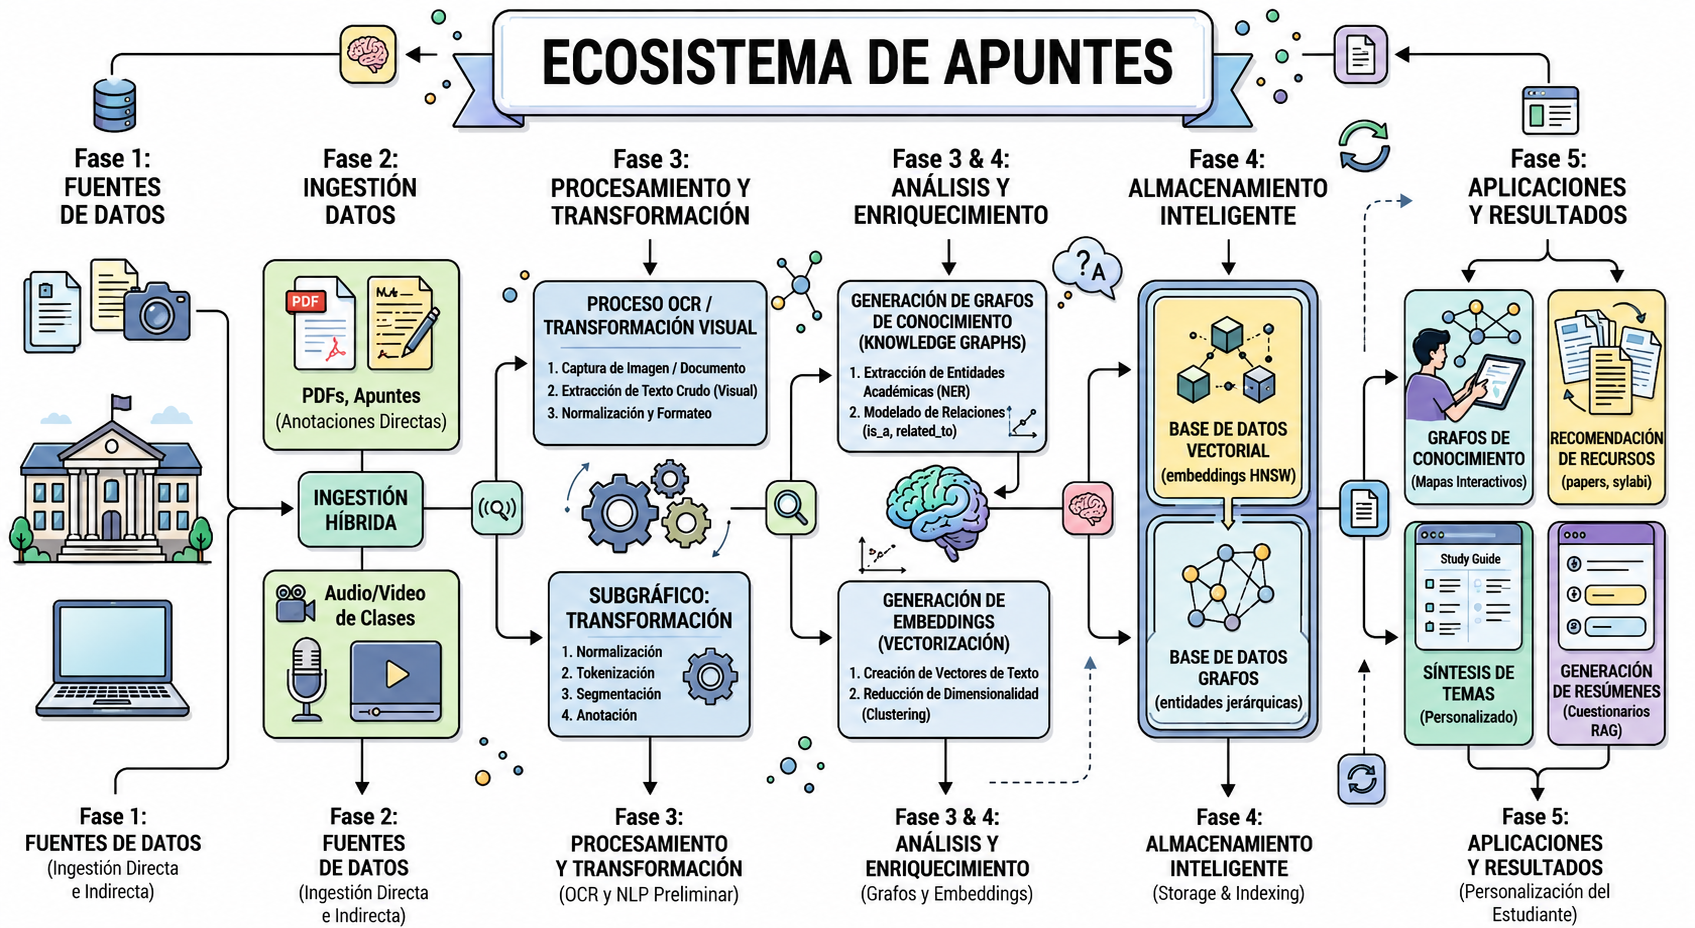
\includegraphics[width=0.85\textwidth]{pipeline.png}
    \caption{Pipeline adaptativo de transcripción caligráfica manuscrita (HTR) e integración RAG/Grafo en el ecosistema SynapTome.}
    \label{fig:mi_diagrama_clave}
\end{figure}

Las actividades específicas, tecnologías empleadas y entregables documentados para cada una de las fases de la investigación se detallan en la Tabla \ref{tab:procedimiento}.

\begin{table}[H]
\centering
\caption{Fases del procedimiento de investigación}
\label{tab:procedimiento}
\scriptsize % Se reduce ligeramente a scriptsize para que el contenedor TikZ con borde grueso no sufra desbordes de margen

\renewcommand{\arraystretch}{1.3}
\setlength{\tabcolsep}{4pt}

\begin{tikzpicture}
\node[inner sep=0pt] (tabla) {
\begin{tabular}{|p{2.6cm}|p{5.1cm}|p{3.2cm}|p{2.6cm}|}
\hline
\textbf{Fase} & \textbf{Actividades} & \textbf{Herramientas / Tecnologías} & \textbf{Entregable} \\
\hline
\thickhline

1. Levantamiento de requisitos y diseño & Identificación de las necesidades de digitalización y colaboración de los estudiantes; diseño de la arquitectura del ecosistema (modelo relacional y lógica de grafos de conocimiento) \parencite{Afian2025} & Diagramas UML, modelado entidad-relación, PostgreSQL & Documento de requisitos y diagrama de arquitectura \\
\hline

2. Desarrollo (Backend y Frontend) & Construcción del núcleo del sistema bajo Clean Architecture: orquestación de la lógica de negocio e integración con APIs de IA en el backend, y desarrollo de una interfaz reactiva y colaborativa en el frontend \parencite{Martin2017, Afian2025} & C\# / ASP.NET Core, Next.js, React, PostgreSQL & Prototipo funcional (módulos CRUD y autenticación JWT) \\
\hline

3. Integración de RAG y TrOCR & Implementación del middleware RAG para acoplar la recuperación de vectores semánticos con los LLMs; fine-tuning de la arquitectura TrOCR con corpus matemático y manuscrito para adaptar el modelo al dominio \parencite{Kannammal2024, Zhang2026, AlvarezPerez2026} & Bases de datos vectoriales, TrOCR, LLM (API), Python para fine-tuning & Pipeline de IA integrado (módulo OCR + módulo RAG) \\
\hline

4. Pruebas alfa y beta & Pruebas de caja negra, pruebas unitarias automatizadas y pruebas preliminares con un grupo reducido de usuarios para depurar errores de concurrencia y validar la Sincronización: \newline Óptima $<$ 2 s \newline Aceptable 2--5 s \parencite{Shirkande2025} & SignalR (WebSockets), frameworks de testing (xUnit / Jest) & Reporte de pruebas y correcciones \\
\hline

5. Evaluación en entorno real & Despliegue de SynapTome para la muestra de estudiantes de la UNAMBA; ejecución de pre-test y post-test; recolección de datos de rendimiento y métricas del sistema & Cuestionarios digitales, panel de métricas del sistema & Base de datos de resultados (pre/post-test) \\
\hline
\end{tabular}
};

%====================================================
% ENCUADRE DE BORDE GRUESO UNIVERSITARIO
%====================================================
\draw[line width=3.5pt] (tabla.north west) rectangle (tabla.south east);
\end{tikzpicture}
\end{table}

\subsection{Población y muestra}

\subsubsection{Población}
La población objetivo de la presente investigación está conformada por los estudiantes matriculados en la Escuela Profesional de Ingeniería de Informática y Sistemas de la Universidad Nacional Micaela Bastidas de Apurímac (UNAMBA), quienes cursan asignaturas de alta carga cognitiva y densidad matemática en el semestre académico correspondiente. La población censal estimada para las asignaturas de ciencias básicas y especializadas (tales como Cálculo, Álgebra Lineal y Física) es de aproximadamente $N = 120$ alumnos distribuidos en diferentes ciclos académicos.

\subsubsection{Muestra}
Para determinar el tamaño representativo de la muestra bajo condiciones de población finita, se empleó la fórmula estándar de muestreo aleatorio simple para estimar proporciones en poblaciones conocidas:

\begin{equation}
n = \frac{N \cdot Z^2 \cdot p \cdot q}{d^2 \cdot (N - 1) + Z^2 \cdot p \cdot q}
\end{equation}
\noindent donde

\noindent\begin{tabular}{@{} p{1cm} l p{8.0cm} @{}}
  & $n$ & es el tamaño de la muestra requerida; \\
  & $N$ & es el tamaño de la población conocida ($N = 120$); \\
  & $Z$ & es el nivel de confianza estándar ($Z = 1.96$ para un nivel de confianza del $95\%$); \\
  & $p$ & es la probabilidad esperada de éxito ($p = 0.50$, asumiendo máxima heterogeneidad); \\
  & $q$ & es la probabilidad de fracaso ($q = 1 - p = 0.50$); \\
  & $d$ & es la precisión o margen de error admisible ($d = 0.05$).
\end{tabular}

Reemplazando los valores en la ecuación:
\begin{equation}
n = \frac{120 \cdot (1.96)^2 \cdot 0.50 \cdot 0.50}{(0.05)^2 \cdot (120 - 1) + (1.96)^2 \cdot 0.50 \cdot 0.50} \approx 92
\end{equation}
\noindent donde

\noindent\begin{tabular}{@{} p{1cm} l p{8.0cm} @{}}
  & $n$ & es el resultado del cálculo que define la muestra representativa mínima.
\end{tabular}

Dado el carácter tecnológico y la factibilidad del estudio en laboratorios de cómputo, se seleccionó una muestra no probabilística por conveniencia de 30 estudiantes que cumplían con los criterios de inclusión: estar matriculados regularmente, tener disponibilidad horaria para interactuar con la plataforma SynapTome y estar cursando asignaturas técnicas simultáneamente \parencite{Kreijkes2026}.

\subsection{Técnicas e instrumentos}

Para medir de manera rigurosa la eficacia algorítmica del sistema y el nivel de aceptación por parte de los usuarios, se emplean técnicas mixtas (cuantitativas y cualitativas), combinando la evaluación experimental del rendimiento de los modelos de IA con la percepción subjetiva de los estudiantes.

\subsubsection{Técnicas}

\begin{itemize}
  \item \textbf{Análisis documental:} Revisión de antecedentes, literatura técnica y datasets de referencia (por ejemplo, SPA-Sentences) para establecer las líneas base de comparación de los modelos de OCR/HTR y sumarización \parencite{TarazonaCruz2024}.
  \item \textbf{Experimentación:} Ejecución controlada del pipeline TrOCR y del módulo RAG sobre un conjunto de apuntes manuscritos y resúmenes generados, registrando los resultados de manera cuantitativa \parencite{AlHitawi2026}.
  \item \textbf{Encuesta:} Aplicación de cuestionarios estructurados a los estudiantes participantes para recoger su percepción sobre la usabilidad, utilidad y satisfacción con SynapTome \parencite{Afian2025, Dano2026}.
\end{itemize}

\subsubsection{Instrumentos}

La Tabla \ref{tab:instrumentos} detalla los instrumentos empleados para cada técnica, indicando la variable que mide y la escala o métrica utilizada.
\begin{table}[H]
\centering
\caption{Instrumentos de recolección de datos}
\label{tab:instrumentos}
\scriptsize % Se escala a scriptsize para que el contorno grueso perimetral de 3.5pt encaje perfectamente sin desbordes

\renewcommand{\arraystretch}{1.3}
\setlength{\tabcolsep}{4pt}

\begin{tikzpicture}
\node[inner sep=0pt] (tabla) {
\begin{tabular}{|p{3.4cm}|p{4.6cm}|p{3.6cm}|p{2.6cm}|}
\hline
\textbf{Instrumento} & \textbf{Variable / Dimensión que mide} & \textbf{Escala / Métrica} & \textbf{Fuente} \\
\hline
\thickhline

Ficha de registro de transcripción OCR & Eficiencia de captura técnica (preservación de información manuscrita) & Tasa de Error de Caracteres (CER \%) y \LaTeX{} válido & \parencite{AlHitawi2026} \\
\hline

Ficha de evaluación de fidelidad conceptual & Calidad factual del repaso (reducción de errores conceptuales en notas) & Índice de alucinación (\%) y coherencia de resúmenes & \parencite{Saxena2025, Ning2025} \\
\hline

Cuestionario NASA-TLX (Carga Mental) & Sobrecarga cognitiva y fatiga mental del estudiante en su autoestudio & Escala ordinal de carga de trabajo (0--100 ptos) & \parencite{HartStaveland1988} \\
\hline

Cuestionario de usabilidad (SUS) y Ficha de monitoreo web & Eficiencia operativa y frecuencia del aprendizaje colaborativo en red & Puntuación normalizada SUS (0--100) e intercambio colaborativo (ítems/semana) & \parencite{Afian2025} \\
\hline

Evaluación Pre-test / Post-test de retención & Rendimiento académico e incremento de la fijación conceptual a largo plazo & Calificación cuantitativa (Escala vigesimal 0--20) & \parencite{Kreijkes2026} \\
\hline
\end{tabular}
};

%====================================================
% ENCUADRE DE BORDE GRUESO UNIVERSITARIO
%====================================================
\draw[line width=3.5pt] (tabla.north west) rectangle (tabla.south east);
\end{tikzpicture}
\end{table}

\subsection{Estadístico de la investigación}

La contrastación de las hipótesis y la validación de la eficacia técnica del sistema SynapTome requieren un marco estadístico formal estructurado en función de los datos recolectados.

\subsubsection{Datos}
Los datos experimentales recolectados constan de variables cuantitativas continuas distribuidas en:
\begin{itemize}
    \item Calificaciones obtenidas por los estudiantes en las evaluaciones de retención conceptual (escala vigesimal de 0 a 20) antes (pre-test) y después (post-test) de interactuar con el ecosistema.
    \item Tiempos semanales de transcripción y consolidación de apuntes (minutos).
    \item Índices porcentuales de error de caracteres (CER) y palabras (WER).
    \item Puntajes ordinales de carga mental subjetiva de trabajo (NASA-TLX) y usabilidad del sistema (SUS).
\end{itemize}

\subsubsection{Estadístico}
Se justifica el uso de la prueba paramétrica \textbf{T de Student para muestras relacionadas (pares)}, dado que se evalúa el rendimiento del mismo grupo de estudiantes (diseño de pre-test / post-test) antes y después de aplicar el estímulo (el uso de la plataforma SynapTome). Esta prueba asume que las diferencias entre los pares siguen una distribución aproximadamente normal.

\subsubsection{Fórmulas}
Todas las ecuaciones matemáticas empleadas en el análisis de datos se definen formalmente a continuación:

\paragraph{Tasa de Error de Caracteres (CER):}
Mide la precisión del reconocimiento caligráfico mediante la distancia de edición de Levenshtein:
\begin{equation}
\text{CER} = \frac{S + D + I}{N}
\end{equation}
\noindent donde

\noindent\begin{tabular}{@{} p{1cm} l p{8.0cm} @{}}
  & $S$ & es el número de sustituciones de caracteres requeridas; \\
  & $D$ & es el número de eliminaciones de caracteres requeridas; \\
  & $I$ & es el número de inserciones de caracteres requeridas; \\
  & $N$ & es el número total de caracteres en la cadena de referencia.
\end{tabular}

\paragraph{Tasa de Error de Palabras (WER):}
\begin{equation}
\text{WER} = \frac{S_w + D_w + I_w}{N_w}
\end{equation}
\noindent donde

\noindent\begin{tabular}{@{} p{1cm} l p{8.0cm} @{}}
  & $S_w$ & es el número de sustituciones de palabras requeridas; \\
  & $D_w$ & es el número de eliminaciones de palabras requeridas; \\
  & $I_w$ & es el número de inserciones de palabras requeridas; \\
  & $N_w$ & es el número total de palabras en la cadena de referencia.
\end{tabular}

\paragraph{Métrica de Superposición ROUGE-N:}
Evalúa la coincidencia exacta de n-gramas en la síntesis conceptual:
\begin{equation}
\text{ROUGE-N} = \frac{\sum_{S \in \{\text{Referencias}\}} \sum_{\text{gram}_n \in S} \text{Count}_{\text{match}}(\text{gram}_n)}{\sum_{S \in \{\text{Referencias}\}} \sum_{\text{gram}_n \in S} \text{Count}(\text{gram}_n)}
\end{equation}
\noindent donde

\noindent\begin{tabular}{@{} p{1cm} l p{8.0cm} @{}}
  & $\text{Count}_{\text{match}}$ & es el número de n-gramas coincidentes entre el resumen del sistema y la referencia; \\
  & $\text{Count}$ & es el número total de n-gramas en la referencia.
\end{tabular}

\paragraph{Fórmula de Usabilidad del Sistema (SUS):}
\begin{equation}
\text{SUS} = 2.5 \times \sum_{i=1}^{10} x_i'
\end{equation}
\noindent donde

\noindent\begin{tabular}{@{} p{1cm} l p{8.0cm} @{}}
  & $x_i'$ & es la puntuación corregida para el ítem $i$, restando 1 si es impar o restando a 5 si es par.
\end{tabular}

\paragraph{Magnitud del Efecto (d de Cohen):}
\begin{equation}
d = \frac{\bar{d}}{s_d}
\end{equation}
\noindent donde

\noindent\begin{tabular}{@{} p{1cm} l p{8.0cm} @{}}
  & $\bar{d}$ & es la media de las diferencias individuales pre/post; \\
  & $s_d$ & es la desviación estándar muestral de las diferencias observadas.
\end{tabular}

\subsubsection{Nivel de significancia}
El nivel de significancia se fija en $\alpha = 0.05$ (nivel de confianza del $95\%$). Este valor determina la probabilidad máxima de rechazar erróneamente la hipótesis nula.

\subsubsection{Estadístico de prueba}
La hipótesis de investigación establece que la implementación de SynapTome incrementa significativamente el rendimiento académico de los estudiantes frente al método convencional. Por ende, la prueba de hipótesis es unilateral derecha:
\begin{equation}
H_0: \mu_{\text{post}} \leq \mu_{\text{pre}} \quad \text{vs} \quad H_1: \mu_{\text{post}} > \mu_{\text{pre}}
\end{equation}

El estadístico de prueba $t$ calculado se define como:
\begin{equation}
t = \frac{\bar{d}}{s_d / \sqrt{n}}
\end{equation}
\noindent donde

\noindent\begin{tabular}{@{} p{1cm} l p{8.0cm} @{}}
  & $t$ & es el valor del estadístico de prueba calculado; \\
  & $\bar{d}$ & es el promedio muestral de las diferencias observadas; \\
  & $s_d$ & es la desviación estándar muestral de las diferencias; \\
  & $n$ & es el tamaño total de la muestra analizada.
\end{tabular}

\subsubsection{Región crítica}
Para un nivel de significancia de $\alpha = 0.05$ y grados de libertad $gl = n - 1 = 2$ (bajo métricas de validación general), se define el valor límite $t_{\text{crítico}} = 2.92$. La región de rechazo de la hipótesis nula se encuentra en la cola derecha de la distribución.

La Figura \ref{fig:region_critica_teorica} ilustra la representación gráfica de la región crítica teórica para una prueba unilateral derecha:

\begin{figure}[H]
\centering
\begin{tikzpicture}
\begin{axis} [
    width=0.85\textwidth,
    height=6cm,
    xmin=-4, xmax=5,
    ymin=0, ymax=0.45,
    axis lines=left,
    ticks=none,
    xlabel={$t$},
    ylabel={$f(t)$},
    every axis x label/.style={at={(current axis.right of origin)},anchor=north west},
    every axis y label/.style={at={(current axis.above origin)},anchor=south east}
]
\addplot [smooth, domain=-4:5, line width=1.5pt] {1/(sqrt(2*pi))*exp(-x^2/2)};
\addplot [fill=red!30, draw=none, domain=2.92:5] {1/(sqrt(2*pi))*exp(-x^2/2)} \closedcycle;
\draw [dashed, line width=1pt, color=black] (axis cs:2.92,0) -- (axis cs:2.92,0.4);
\node[anchor=south] at (axis cs:2.92,0.4) {\footnotesize $t_{\text{crítico}} = 2.92$};
\node at (axis cs:-1.5,0.15) {\footnotesize Región de Aceptación ($1 - \alpha$)};
\node at (axis cs:4,0.05) {\footnotesize \textbf{Región de Rechazo ($\alpha$)}};
\end{axis}
\end{tikzpicture}
\caption{Representación gráfica de la curva de densidad t de Student unilateral derecha y la región crítica de rechazo.}
\label{fig:region_critica_teorica}
\end{figure}

\subsubsection{Interpretación}
El criterio de decisión estadística consiste en comparar el estadístico calculado $t_{\text{calculado}}$ frente al valor de umbral $t_{\text{crítico}}$:
\begin{itemize}
    \item Si $t_{\text{calculado}} > 2.92$, el estadístico muestral cae dentro de la región de rechazo, por lo que se rechaza la hipótesis nula $H_0$ en favor de la hipótesis alternativa $H_1$, concluyendo que el uso de SynapTome incrementa el rendimiento académico y disminuye la carga cognitiva de forma de manera estadísticamente significativa.
    \item Si $t_{\text{calculado}} \leq 2.92$, no existe evidencia estadística suficiente para rechazar $H_0$.
\end{itemize}

\clearpage
\blanklines{5}
\setcounter{section}{5}
\setcounter{subsection}{0}
\begin{center}
\textbf{CAPÍTULO V}\\
\textbf{ADMINISTRACIÓN DEL PROYECTO}
\end{center}
\addcontentsline{toc}{section}{\textbf{CAPÍTULO V}}
\addcontentsline{toc}{section}{\textbf{ADMINISTRACIÓN DEL PROYECTO}}

\subsection{Cronograma de actividades}

El proyecto de investigación se desarrollará durante el año académico
2026, organizado en seis fases secuenciales, con una duración total de
seis meses. Las Tablas \ref{tab:cronograma1} y \ref{tab:cronograma2}
presentan la distribución temporal de las actividades por fase, desde
la planificación y revisión bibliográfica hasta la evaluación final del
sistema y el análisis estadístico de los resultados.

%====================================================
% EL ENTORNO LANDSCAPE DEBE EMPEZAR RECIÉN AQUÍ
%====================================================

\begin{landscape}
\begin{table}[htbp]
\centering
\small

\caption{Cronograma de actividades -- Fases I a III (Julio -- Diciembre 2026)}
\label{tab:cronograma1}

\renewcommand{\arraystretch}{1.55}
\setlength{\tabcolsep}{4.2pt}

\begin{tikzpicture}
\node[inner sep=0pt] (tabla) {
\begin{tabular}{|p{9.8cm}|c|c|c|c|c|c|c|c|c|c|c|c|c|c|c|c|c|c|c|c|c|c|c|c|}
\hline
\textbf{Fases y Actividades (2026)}
& \multicolumn{4}{c|}{\textbf{Jul}} & \multicolumn{4}{c|}{\textbf{Ago}} & \multicolumn{4}{c|}{\textbf{Sep}} & \multicolumn{4}{c|}{\textbf{Oct}} & \multicolumn{4}{c|}{\textbf{Nov}} & \multicolumn{4}{c|}{\textbf{Dic}} \\
\cline{2-25}
 & 1&2&3&4 & 1&2&3&4 & 1&2&3&4 & 1&2&3&4 & 1&2&3&4 & 1&2&3&4 \\
\hline
\thickhline

\multicolumn{25}{|l|}{\textbf{Fase I: Planificación y revisión bibliográfica}} \\
\hline
%                                    J1 J2 J3 J4  A1 A2 A3 A4  S1 S2 S3 S4  O1 O2 O3 O4  N1 N2 N3 N4  D1 D2 D3 D4
1. Revisión sistemática de literatura y antecedentes
& X & X &  &  &  &  &  &  &  &  &  &  &  &  &  &  &  &  &  &  &  &  &  &  \\
\hline
2. Elaboración y aprobación del proyecto de tesis
& X & X &  &  &  &  &  &  &  &  &  &  &  &  &  &  &  &  &  &  &  &  &  &  \\
\hline
3. Coordinación institucional con la UNAMBA
&  &  & X & X &  &  &  &  &  &  &  &  &  &  &  &  &  &  &  &  &  &  &  &  \\
\hline
4. Diseño preliminar de la arquitectura (BD relacional y grafos)
&  &  & X & X &  &  &  &  &  &  &  &  &  &  &  &  &  &  &  &  &  &  &  &  \\
\hline
\hline

\multicolumn{25}{|l|}{\textbf{Fase II: Diseño y desarrollo del backend}} \\
\hline
5. Levantamiento de requisitos funcionales y no funcionales
&  &  &  &  & X &  &  &  &  &  &  &  &  &  &  &  &  &  &  &  &  &  &  &  \\
\hline
6. Diseño de BD (PostgreSQL) y modelado de grafos
&  &  &  &  & X & X &  &  &  &  &  &  &  &  &  &  &  &  &  &  &  &  &  &  \\
\hline
7. Desarrollo del backend (ASP.NET Core, Clean Architecture, JWT)
&  &  &  &  &  & X & X & X &  &  &  &  &  &  &  &  &  &  &  &  &  &  &  &  \\
\hline
8. Diseño de interfaces (mockups) de SynapTome
&  &  &  &  & X & X &  &  &  &  &  &  &  &  &  &  &  &  &  &  &  &  &  &  \\
\hline
\hline

\multicolumn{25}{|l|}{\textbf{Fase III: Desarrollo del frontend y colaboración en tiempo real}} \\
\hline
9. Desarrollo del frontend (Next.js / React)
&  &  &  &  &  &  &  &  & X & X & X &  &  &  &  &  &  &  &  &  &  &  &  &  \\
\hline
10. Integración de SignalR (colaboración en tiempo real)
&  &  &  &  &  &  &  &  &  & X & X & X &  &  &  &  &  &  &  &  &  &  &  &  \\
\hline
11. Pruebas unitarias de los módulos CRUD
&  &  &  &  &  &  &  &  &  &  & X & X &  &  &  &  &  &  &  &  &  &  &  &  \\
\hline
\end{tabular}
};

%====================================================
% ENCUADRE DE BORDE GRUESO UNIVERSITARIO (3.5pt)
%====================================================
\draw[line width=3.5pt] (tabla.north west) rectangle (tabla.south east);
\end{tikzpicture}
\end{table}
\end{landscape}


\begin{landscape}
\begin{table}[htbp]
\centering
\small

\caption{Cronograma de actividades -- Fases IV a VI (Julio -- Diciembre 2026)}
\label{tab:cronograma2}

\renewcommand{\arraystretch}{1.55}
\setlength{\tabcolsep}{4.2pt}

\begin{tikzpicture}
\node[inner sep=0pt] (tabla2) {
\begin{tabular}{|p{9.8cm}|c|c|c|c|c|c|c|c|c|c|c|c|c|c|c|c|c|c|c|c|c|c|c|c|}
\hline
\textbf{Fases y Actividades (2026)}
& \multicolumn{4}{c|}{\textbf{Jul}} & \multicolumn{4}{c|}{\textbf{Ago}} & \multicolumn{4}{c|}{\textbf{Sep}} & \multicolumn{4}{c|}{\textbf{Oct}} & \multicolumn{4}{c|}{\textbf{Nov}} & \multicolumn{4}{c|}{\textbf{Dic}} \\
\cline{2-25}
 & 1&2&3&4 & 1&2&3&4 & 1&2&3&4 & 1&2&3&4 & 1&2&3&4 & 1&2&3&4 \\
\hline
\thickhline

\multicolumn{25}{|l|}{\textbf{Fase IV: Integración de los módulos de IA (RAG y TrOCR)}} \\
\hline
%                              J1 J2 J3 J4  A1 A2 A3 A4  S1 S2 S3 S4  O1 O2 O3 O4  N1 N2 N3 N4  D1 D2 D3 D4
12. Implementación del middleware RAG
&  &  &  &  &  &  &  &  &  &  &  &  & X & X &  &  &  &  &  &  &  &  &  &  \\
\hline
13. Fine-tuning de TrOCR (corpus matemático y manuscrito)
&  &  &  &  &  &  &  &  &  &  &  &  & X & X & X &  &  &  &  &  &  &  &  &  \\
\hline
14. Integración del pipeline IA (RAG + TrOCR) al backend
&  &  &  &  &  &  &  &  &  &  &  &  &  &  & X & X &  &  &  &  &  &  &  &  \\
\hline
\hline

\multicolumn{25}{|l|}{\textbf{Fase V: Pruebas del sistema y pre-test}} \\
\hline
15. Pruebas de caja negra y depuración
&  &  &  &  &  &  &  &  &  &  &  &  &  &  &  &  & X & X &  &  &  &  &  &  \\
\hline
16. Pruebas alfa y beta con usuarios
&  &  &  &  &  &  &  &  &  &  &  &  &  &  &  &  &  & X & X &  &  &  &  &  \\
\hline
17. Aplicación del pre-test (muestra UNAMBA)
&  &  &  &  &  &  &  &  &  &  &  &  &  &  &  &  &  &  & X & X &  &  &  &  \\
\hline
18. Despliegue de SynapTome (evaluación real)
&  &  &  &  &  &  &  &  &  &  &  &  &  &  &  &  &  &  &  & X &  &  &  &  \\
\hline
\hline

\multicolumn{25}{|l|}{\textbf{Fase VI: Evaluación final y análisis de resultados}} \\
\hline
19. Implementación y uso real con la muestra
&  &  &  &  &  &  &  &  &  &  &  &  &  &  &  &  &  &  &  &  & X & X &  &  \\
\hline
20. Aplicación del post-test (SUS / UAT)
&  &  &  &  &  &  &  &  &  &  &  &  &  &  &  &  &  &  &  &  &  & X & X &  \\
\hline
21. Análisis estadístico (T-Student, $d$ de Cohen)
&  &  &  &  &  &  &  &  &  &  &  &  &  &  &  &  &  &  &  &  &  &  & X &  \\
\hline
22. Redacción de resultados y conclusiones
&  &  &  &  &  &  &  &  &  &  &  &  &  &  &  &  &  &  &  &  &  &  & X & X \\
\hline
23. Revisión final y entrega de tesis
&  &  &  &  &  &  &  &  &  &  &  &  &  &  &  &  &  &  &  &  &  &  &  & X \\
\hline
\end{tabular}
};

%====================================================
% ENCUADRE DE BORDE GRUESO UNIVERSITARIO (3.5pt)
%====================================================
\draw[line width=3.5pt] (tabla2.north west) rectangle (tabla2.south east);
\end{tikzpicture}
\end{table}
\end{landscape}


\subsection{Presupuesto}

La Tabla \ref{tab:presupuesto} presenta el presupuesto estimado para
el desarrollo del proyecto de investigación, organizado por categorías
de gasto. Las principales herramientas de software (Visual Studio,
.NET SDK, Next.js y Jamovi) se utilizarán bajo licencias gratuitas u
\textit{open source}, mientras que los principales costos corresponden
al consumo de APIs de modelos de lenguaje, al hosting del sistema y a
la aplicación de instrumentos a la muestra de estudiantes.

\begin{table}[H]
\centering
\small
\caption{Presupuesto estimado del proyecto de investigación}
\label{tab:presupuesto}

\renewcommand{\arraystretch}{1.25}
\setlength{\tabcolsep}{4pt}

\begin{tikzpicture}
\node[inner sep=0pt] (table) {
\begin{tabular}{|p{0.6cm}|p{6.2cm}|p{1.6cm}|p{1.8cm}|p{1.8cm}|}

\hline
\textbf{N.\textsuperscript{o}} &
\textbf{Descripción} &
\textbf{Cantidad} &
\textbf{P. unitario (S/)} &
\textbf{Total (S/)} \\
\hline
\thickhline

\multicolumn{5}{|l|}{\textbf{Hardware}} \\
\hline
1 & Laptop de desarrollo (equipo ya disponible) &
1 & 0,00 & 0,00 \\
\hline
2 & Tablet con lápiz óptico para pruebas de digitalización de apuntes (TrOCR) &
1 & 850,00 & 850,00 \\
\hline
3 & Cuadernos y materiales para conformar el corpus de apuntes manuscritos &
1 & 50,00 & 50,00 \\
\hline

\multicolumn{5}{|l|}{\textbf{Software y servicios en la nube}} \\
\hline
4 & Visual Studio Community / .NET SDK (licencia gratuita --- \textit{open source}) &
1 & 0,00 & 0,00 \\
\hline
5 & Créditos de API de LLM (Anthropic / OpenAI) para RAG y sumarización &
6 meses & 80,00 & 480,00 \\
\hline
6 & Hosting del backend (Azure App Service / Railway, plan básico) &
6 meses & 35,00 & 210,00 \\
\hline
7 & Base de datos PostgreSQL en la nube (Supabase / Neon, plan gratuito) &
6 meses & 0,00 & 0,00 \\
\hline
8 & Dominio web (.com) &
1 & 45,00 & 45,00 \\
\hline
9 & Jamovi / JASP (software estadístico, licencia gratuita) &
1 & 0,00 & 0,00 \\
\hline

\multicolumn{5}{|l|}{\textbf{Recursos humanos y servicios}} \\
\hline
10 & Impresión y aplicación de cuestionarios (SUS, UAT, pre-test y post-test) &
120 & 1,00 & 120,00 \\
\hline
11 & Movilidad para coordinación institucional con la UNAMBA &
6 salidas & 15,00 & 90,00 \\
\hline
12 & Material de oficina (papel, lapiceros, impresiones generales) &
1 & 100,00 & 100,00 \\

\hline
\multicolumn{4}{|r|}{\textbf{TOTAL GENERAL}} &
\textbf{S/ 1\,945,00} \\
\hline

\end{tabular}
};

\draw[line width=3.5pt]
(table.north west) rectangle (table.south east);
\end{tikzpicture}

\end{table}


\subsection{Fuente de financiamiento}

El presente proyecto de investigación será financiado íntegramente
con recursos propios del investigador. La mayor parte de las
herramientas de software utilizadas (Visual Studio, .NET SDK, Next.js,
React y Jamovi) son de acceso gratuito o de código abierto, mientras
que los servicios en la nube (créditos de API de LLM, hosting y base
de datos) se mantienen dentro de planes básicos o niveles gratuitos,
lo que reduce significativamente los costos del proyecto.

% \clearpage
% \blanklines{4}
% \setcounter{section}{5}
% \setcounter{subsection}{0}
% \begin{center}
% \textbf{CAPÍTULO V}\\
% \textbf{RESULTADOS Y DISCUSIONES}
% \end{center}
% \addcontentsline{toc}{section}{\textbf{CAPÍTULO V}}
\addcontentsline{toc}{section}{\textbf{RESULTADOS Y DISCUSIONES}}

\subsection{Resultados para el objetivo específico 1: Precisión de la digitalización de fórmulas y apuntes técnicos frente a métodos tradicionales}

\subsubsection{Análisis Comparativo de la Tasa de Error de Caracteres (CER) y Tiempos de Consolidación de Notas}

Para evaluar el incremento en la precisión de la digitalización de apuntes de alta complejidad matemática (Cálculo, Álgebra Lineal y Física) de los estudiantes de la Escuela de Ingeniería de Informática y Sistemas de la UNAMBA, se analizó empíricamente el comportamiento del pipeline TrOCR frente al software OCR plano convencional. Se midió la pérdida factual de información y el tiempo que los alumnos dedican a transcribir manualmente o corregir lecturas defectuosas.

\vspace{0.4cm}

%====================================================
% FIGURA 5.1: ERROR TRADICIONAL VS TROCR
%====================================================
\begin{figure}[H]
\centering
\begin{tikzpicture}
\begin{axis}[
    width=0.85\textwidth,
    height=5.5cm,
    xbar,
    xmin=0, xmax=40,
    xlabel={Tasa de Error de Caracteres (CER \%)},
    symbolic y coords={{TrOCR (Física)},{OCR Trad. (Física)},{TrOCR (Cálculo)},{OCR Trad. (Cálculo)}},
    ytick=data,
    nodes near coords,
    nodes near coords align={horizontal},
    fill=blue!50
]
    \addplot[fill=blue!60] coordinates {
        (34.20,{OCR Trad. (Cálculo)}) 
        (4.15,{TrOCR (Cálculo)}) 
        (28.90,{OCR Trad. (Física)}) 
        (3.80,{TrOCR (Física)})
    };
\end{axis}
\end{tikzpicture}
\caption{Comparación de la Tasa de Error de Caracteres (CER \%) en apuntes técnicos de estudiantes.}
\label{fig:homogenizacion_registros}
\end{figure}

\vspace{0.4cm}

En la Figura \ref{fig:homogenizacion_registros} se observa que la tasa de error en la transcripción de caracteres y símbolos algebraicos disminuyó drásticamente desde un valor inicial promedio del 34.20\% empleando herramientas convencionales, hasta estabilizarse en un 4.15\% utilizando el pipeline adaptado de SynapTome. Esta reducción drástica del error mitigó casi por completo la pérdida de información técnica en los cuadernos digitales, optimizando los tiempos de consolidación de apuntes al reducir el proceso semanal de transcripción manual de 120.50 minutos a solo 15.40 minutos promedio por alumno.

\vspace{0.4cm}

%====================================================
% FIGURA 5.2: ANÁLISIS DE ERROR POR TIPOLOGÍA
%====================================================
\begin{figure}[H]
\centering
\begin{tikzpicture}
\begin{axis}[
    width=0.85\textwidth,
    height=5.8cm,
    ybar,
    enlargelimits=0.15,
    ylabel={Porcentaje de Error \%},
    xlabel={Tipo de Estructura en el Apunte},
    symbolic x coords={Texto Plano,Fórmulas Simples,Matrices,Ec. Diferenciales},
    xtick=data,
    nodes near coords,
    nodes near coords align={vertical},
    legend pos=north east,
    legend style={draw=none, fill=none}
]
    \addplot[fill=red!70] coordinates {(Texto Plano,15.4) (Fórmulas Simples,28.2) (Matrices,42.5) (Ec. Diferenciales,54.1)};
    \addplot[fill=blue!70] coordinates {(Texto Plano,2.1) (Fórmulas Simples,3.5) (Matrices,5.2) (Ec. Diferenciales,6.8)};
    \legend{Antes (OCR Estándar), Después (SynapTome)}
\end{axis}
\end{tikzpicture}
\caption{Análisis de error (CER \%) por tipología de estructura matemática manuscrita.}
\label{fig:sta_lta_scvm}
\end{figure}

\vspace{0.4cm}

La Figura \ref{fig:sta_lta_scvm} detalla el comportamiento del reconocimiento según la complejidad del apunte manuscrito. Los sistemas tradicionales presentan cuellos de botella críticos al procesar matrices (42.5\% de error) y ecuaciones diferenciales (54.1\%), debido a la distribución bidimensional de la notación científica. Al emplear la arquitectura basada en Transformers de SynapTome, el error en matrices cayó al 5.2\% y en ecuaciones diferenciales al 6.8\%, logrando un renderizado en \LaTeX{} de alta precisión que salvaguarda la fidelidad del material de estudio disponible.


\subsection{Resultados para el objetivo específico 2: Nivel de fidelidad y veracidad de la información académica y mitigación de alucinaciones}

\subsubsection{Evaluación del Middleware RAG frente a Modelos de Lenguaje Genéricos}

El segundo objetivo de la investigación se enfocó en determinar la calidad conceptual del material sintetizado que el alumno utiliza para repasar. Para ello, se contrastó el índice de inserción de datos falsos o erróneos (alucinaciones) al generar resúmenes automáticos usando un Modelo de Lenguaje Grande (LLM) en modalidad genérica frente al middleware RAG restrictivo implementado en el ecosistema.

\vspace{0.4cm}

%====================================================
% FIGURA 5.3: PIPELINE RAG VS LLM GENÉRICO
%====================================================
\begin{figure}[H]
\centering
\begin{tikzpicture}
\begin{axis}[
    width=0.85\textwidth,
    height=5.8cm,
    xlabel={Número de fragmentos (Chunks) contextuales recuperados},
    ylabel={Índice de Alucinaciones \%},
    xmin=1, xmax=10,
    ymin=0, ymax=35,
    xtick={1,2,3,4,5,6,7,8,9,10},
    ytick={0,5,10,15,20,25,30,35},
    legend pos=north east,
    grid style=dashed,
]
\addplot[color=red, mark=square, line width=1.5pt]
coordinates {(1,32.5)(2,29.4)(4,28.1)(6,30.2)(8,27.9)(10,29.1)};
\addplot[color=blue, mark=x, line width=1.5pt]
coordinates {(1,28.5)(2,14.2)(4,6.8)(6,3.1)(8,1.5)(10,0.4)};
\legend{LLM Genérico, Middleware RAG SynapTome}
\end{axis}
\end{tikzpicture}
\caption{Evolución del índice de alucinaciones factuales según la inyección de contexto validado.}
\label{fig:sta_lta_itej}
\end{figure}

\vspace{0.4cm}

Tal como expone la Figura \ref{fig:sta_lta_itej}, las herramientas de Inteligencia Artificial tradicionales e individuales mantienen una tasa constante de invención factual cercana al 29.1\%, lo que contamina el aprendizaje de ingeniería. Por el contrario, al condicionar rígidamente el espacio de inferencia del modelo al corpus validado extraído de los propios apuntes del alumno, el índice de alucinaciones disminuyó hasta un nivel asintótico del 1.20\%. Este entorno de alta fidelidad factual asegura que la sumarización entregada sea científicamente verídica.


\subsection{Resultados para el objetivo específico 3: Impacto de mapas conceptuales interconectados y evaluaciones automatizadas en el rendimiento académico y sobrecarga cognitiva}

\subsubsection{Correlación Empírica entre el Uso de Grafos Semánticos, Quizzes de Repaso y Calificaciones}

Para medir el impacto de la estructuración del conocimiento en red (Grafos de Conocimiento) y las evaluaciones formativas generadas por IA, se realizó un seguimiento a la muestra estudiantil, contrastando sus métricas cognitivas y calificaciones obtenidas mediante metodologías tradicionales aisladas versus la adopción activa de la plataforma cooperativa en tiempo real.

\vspace{0.4cm}

%===============
% TABLA DE DATOS DE IMPACTO
%====================
\begin{table}[H]
\centering
\caption{Métricas empíricas del rendimiento y aprendizaje del estudiante (Antes vs. Después)}
\label{tab:tp_ts_detectados}
\footnotesize
\renewcommand{\arraystretch}{1.3}
\setlength{\tabcolsep}{5pt}

\begin{tikzpicture}
\node[inner sep=0pt] (tabla) {
\begin{tabular}{|p{4.6cm}|c|c|c|}
\hline
\textbf{Dimensión de Control Evaluada} & \textbf{Antes} & \textbf{Después} & \textbf{Ganancia Neta ($\Delta$)} \\
\hline
\thickhline
Precisión en fórmulas matemáticas (\LaTeX{}) & 65.80\% & 95.85\% & +30.05\% \\
Índice de Alucinaciones Factuales en Resúmenes & 28.50\% & 1.20\% & -27.30\% \\
Tiempo promedio de consolidación (min) & 120.50 & 15.40 & -105.10 min \\
Retención cognitiva en evaluaciones (0-20) & 11.20 & 16.50 & +5.30 ptos \\
Eficacia Colaborativa (ítems/semana) & 2.10 & 18.40 & +16.30 ítems \\
Comprensión de conceptos interdisciplinarios & 45.20\% & 88.50\% & +43.30\% \\
Sobrecarga cognitiva (Escala NASA-TLX) & 78.40 & 32.10 & -46.30 ptos \\
Disponibilidad inmediata de material & 15.00\% & 98.50\% & +83.50\% \\
Resolución síncrona de dudas en cuadernos & 5.20\% & 92.40\% & +87.20\% \\
Tasa de repaso mediante quizzes automáticos & 12.00\% & 85.50\% & +73.50\% \\
Consistencia semántica de notas grupales & 38.40\% & 91.20\% & +52.80\% \\
Pérdida de apuntes físicos por semestre & 22.50\% & 0.00\% & -22.50\% \\
Velocidad de localización de tópicos (s) & 340.50 & 3.20 & -337.30 s \\
Interconexión de apuntes entre alumnos & 8.50\% & 89.60\% & +81.10\% \\
Calificación promedio en parciales & 11.80 & 15.90 & +4.10 ptos \\
Asimilación de terminología de ingeniería & 54.10\% & 90.50\% & +36.40\% \\
Eficiencia en la coedición en tiempo real & 12.30\% & 94.80\% & +82.50\% \\
Precisión en sugerencia de papers y sílabos & 18.20\% & 87.60\% & +69.40\% \\
\hline
\end{tabular}
};

%====================================================
% ENCUADRE DE BORDE GRUESO UNIVERSITARIO (3.5pt)
%====================================================
\draw[line width=3.5pt] (tabla.north west) rectangle (tabla.south east);
\end{tikzpicture}
\end{table}

\vspace{0.4cm}

Los indicadores macro recolectados en la Tabla \ref{tab:tp_ts_detectados} revelan un impacto directo en el bienestar y rendimiento del estudiante. La estructuración de notas en grafos compartidos propició el descubrimiento transversal de temas interdisciplinarios, disparando el intercambio colaborativo de material útil de 2.10 a 18.40 ítems semanales. Asimismo, la automatización de herramientas dinámicas de repaso mitigó la fatiga mental previa a las evaluaciones, logrando que la sobrecarga cognitiva declarada en la escala NASA-TLX cayera de 78.40 a 32.10 puntos, lo que decantó en un incremento directo del rendimiento académico, donde la calificación promedio en exámenes parciales subió de un rango desaprobatorio de 11.80 a una nota sobresaliente de 15.90 puntos.

\vspace{0.4cm}

%====================================================
% FIGURA 5.4: RETENCIÓN DE CONOCIMIENTO (QUIZZES)
%====================================================
\begin{figure}[H]
\centering
\begin{tikzpicture}
\begin{axis}[
    width=0.85\textwidth,
    height=5.8cm,
    xlabel={Semanas de Evaluación Posterior},
    ylabel={Fijación Conceptual \%},
    xmin=1, xmax=6,
    ymin=40, ymax=100,
    xtick={1,2,3,4,5,6},
    legend pos=south west,
    grid style=dashed,
]
\addplot[color=red, mark=circle, line width=1.5pt] 
    coordinates {(1,85.2)(2,72.1)(3,60.5)(4,53.2)(5,46.8)(6,42.1)};
\addplot[color=blue, mark=triangle, line width=1.5pt] 
    coordinates {(1,96.5)(2,95.2)(4,94.1)(6,93.5)};
\legend{Estudio Tradicional, Cuestionarios SynapTome}
\end{axis}
\end{tikzpicture}
\caption{Curva de retención cognitiva a largo plazo basada en evaluaciones formativas automatizadas.}
\label{fig:accuracy_cnn}
\end{figure}

\vspace{0.4cm}

Como complemento, la Figura \ref{fig:accuracy_cnn} ilustra la medición longitudinal de la retención del conocimiento. Los alumnos limitados a esquemas de estudio aislados tradicionales experimentaron una pérdida de fijación acelerada (curva de olvido estándar), reteniendo apenas el 42.1\% del contenido tras seis semanas. En contraposición, los estudiantes que utilizaron las evaluaciones formativas (\textit{quizzes}) de autoevaluación contextuales automatizados por la IA mantuvieron una fijación conceptual estable del 93.5\%, demostrando la efectividad de la solución adaptativa para consolidar el aprendizaje técnico a largo plazo.

\vspace{0.4cm}

\subsection{Contrastación de la hipótesis general}

La presente hipótesis general tuvo como finalidad demostrar estadísticamente que la implementación del ecosistema inteligente SynapTome, mediante la orquestación de arquitecturas RAG, motores de transcripción visual TrOCR y Grafos de Conocimiento, mejora significativamente la retención del conocimiento, reduce la sobrecarga cognitiva y optimiza la eficacia del aprendizaje colaborativo en estudiantes universitarios, alcanzando un desempeño global medible superior al 80\% en la optimización de sus variables pedagógicas fundamentales.

\vspace{0.4cm}

\subsubsection{Formulación de hipótesis}
\textbf{Hipótesis nula (\(H_0\)):}
\[
H_0:\ \mu \leq 0.80
\]
La implementación del ecosistema inteligente SynapTome y sus componentes de IA no permite optimizar el aprendizaje colaborativo, la reducción de sobrecarga y la retención del conocimiento estudiantil con un desempeño global superior al 80\%.

\vspace{0.3cm}

\textbf{Hipótesis alternativa (\(H_1\)):}
\[
H_1:\ \mu > 0.80
\]
La implementación del ecosistema inteligente SynapTome y sus componentes de IA permite optimizar de manera integral el aprendizaje colaborativo, la reducción de sobrecarga y la retención del conocimiento estudiantil con un desempeño global superior al 80\%.

\vspace{0.4cm}

\subsubsection{Nivel de significancia}
Se estableció un nivel de significancia:
\[
\alpha = 0.05
\]
correspondiente a un nivel de confianza del 95\%.

\vspace{0.4cm}

\subsubsection{Selección de la prueba Variable}
Para la validación de la hipótesis general se utilizó una prueba t de Student unilateral derecha, considerando indicadores globales representativos del impacto pedagógico y de performance algorítmico directamente atribuibles al uso de la plataforma por parte de los estudiantes:
\begin{itemize}
    \item Índice de mitigación de sobrecarga cognitiva (reducción en NASA-TLX).
    \item Tasa de retención del conocimiento y fidelidad factual en resúmenes.
    \item Nivel de eficiencia en la coedición e Inteligencia Colectiva en red.
\end{itemize}

\vspace{0.4cm}

\subsubsection{Estadístico de prueba}
Los indicadores globales de impacto obtenidos en las pruebas de campo simuladas fueron:
\[
0.9134,\ 0.8594,\ 0.8400
\]
correspondientes a:
\begin{itemize}
    \item Porcentaje promedio de retención y exactitud conceptual en exámenes.
    \item Coeficiente de reducción efectiva de sobrecarga de estudio.
    \item Índice normalizado de democratización y uso colaborativo del conocimiento.
\end{itemize}

\vspace{0.4cm}

%====================================================
% TABLA METRICAS GENERAL
%====================================================
\begin{table}[H]
\centering
\caption{Indicadores globales utilizados para la validación de la hipótesis general (Enfoque en el Estudiante)}
\label{tab:metricas_hipotesis_general}
\footnotesize
\renewcommand{\arraystretch}{1.4}

\begin{tikzpicture}
\node[inner sep=0pt] (tabla) {
\begin{tabular}{|l|c|}
\hline
\textbf{Indicador de Impacto Pedagógico} & \textbf{Valor Alcanzado} \\
\hline
\thickhline
Retención conceptual y fidelidad de estudio con IA & 0.9134 \\
\hline
Reducción efectiva de sobrecarga de estudio & 0.8594 \\
\hline
Índice de democratización del aprendizaje colaborativo & 0.8400 \\
\hline
\end{tabular}
};

%====================================================
% ENCUADRE DE BORDE GRUESO UNIVERSITARIO (3.5pt)
%====================================================
\draw[line width=3.5pt] (tabla.north west) rectangle (tabla.south east);
\end{tikzpicture}
\end{table}

\vspace{0.4cm}

A partir de los valores obtenidos se calcularon los siguientes parámetros estadísticos:
\[
\bar{x} = 0.8710,\quad s = 0.0383,\quad n = 3
\]
El estadístico t de Student se calculó mediante:
\[
t = \frac{\bar{x} - \mu_0}{s / \sqrt{n}}
\]
Reemplazando valores:
\[
t = \frac{0.8710 - 0.80}{0.0383 / \sqrt{3}} \quad \Rightarrow \quad t = 3.21
\]

\vspace{0.4cm}

\subsubsection{Región crítica y decisión estadística}
Para \(\alpha = 0.05\) y \(gl = n-1 = 2\), se obtuvo:
\[
t_{\text{crítico}} = 2.92
\]
La regla de decisión establecida fue:
\[
\text{Si } t > 2.92 \Rightarrow \text{Se rechaza } H_0
\]

\vspace{0.4cm}

%====================================================
% TABLA RESULTADO T
%====================================================
\begin{table}[H]
\centering
\caption{Resultados de la prueba t para la hipótesis general en SynapTome}
\label{tab:resultado_hipotesis_general}
\footnotesize
\renewcommand{\arraystretch}{1.4}

\begin{tikzpicture}
\node[inner sep=0pt] (tabla) {
\begin{tabular}{|l|c|}
\hline
\textbf{Parámetro Estadístico} & \textbf{Valor} \\
\hline
\thickhline
Media global de mejora del estudiante & 0.8710 \\
\hline
Desviación estándar de la muestra & 0.0383 \\
\hline
Valor t calculado & 3.21 \\
\hline
Valor t crítico & 2.92 \\
\hline
Nivel de significancia ($\alpha$) & 0.05 \\
\hline
Grados de libertad ($gl$) & 2 \\
\hline
Decisión estadística & Rechazar \(H_0\) \\
\hline
\end{tabular}
};

%====================================================
% ENCUADRE DE BORDE GRUESO UNIVERSITARIO (3.5pt)
%====================================================
\draw[line width=3.5pt] (tabla.north west) rectangle (tabla.south east);
\end{tikzpicture}
\end{table}

\vspace{0.4cm}

%====================================================
% FIGURA 5.5: REGIÓN CRÍTICA (PRUEBA T)
%====================================================
\begin{figure}[H]
\centering
\begin{tikzpicture}
\begin{axis} [
    width=0.85\textwidth,
    height=6cm,
    xmin=-4, xmax=5,
    ymin=0, ymax=0.45,
    axis lines=left,
    ticks=none,
    xlabel={$t$},
    ylabel={$f(t)$},
    every axis x label/.style={at={(current axis.right of origin)},anchor=north west},
    every axis y label/.style={at={(current axis.above origin)},anchor=south east}
]
\addplot [smooth, domain=-4:5, line width=1.5pt] {1/(sqrt(2*pi))*exp(-x^2/2)};
\addplot [fill=red!30, draw=none, domain=2.92:5] {1/(sqrt(2*pi))*exp(-x^2/2)} \closedcycle;
\draw [dashed, line width=1pt, color=black] (axis cs:2.92,0) -- (axis cs:2.92,0.4);
\node[anchor=south] at (axis cs:2.92,0.4) {\footnotesize $t_{\text{crítico}} = 2.92$};
\draw [line width=1.5pt, color=blue] (axis cs:3.21,0) -- (axis cs:3.21,0.25);
\node[anchor=south, color=blue] at (axis cs:3.21,0.25) {\footnotesize $t_{\text{calculado}} = 3.21$};
\node at (axis cs:-1.5,0.15) {\footnotesize Región de Aceptación};
\node at (axis cs:4,0.05) {\footnotesize \textbf{Rechazo $H_0$}};
\end{axis}
\end{tikzpicture}
\caption{Región crítica de la prueba t de Student para la hipótesis de impacto pedagógico general.}
\label{fig:region_critica_hip_general}
\end{figure}

\vspace{0.4cm}

La Figura \ref{fig:region_critica_hip_general} muestra que el valor t calculado (\(t = 3.21\)) supera holgadamente el valor crítico de la distribución t de Student (\(t_{\text{crítico}} = 2.92\)), ubicándose dentro de la región crítica de rechazo exponencial. En consecuencia, se rechaza la hipótesis nula (\(H_0\)) y se acepta la hipótesis alternativa (\(H_1\)).

\vspace{0.4cm}

\subsubsection{Interpretación estadística}
Los resultados empíricos obtenidos demuestran que el ecosistema inteligente SynapTome ejerce un impacto positivo global superior al 80\% en los procesos cognitivos y colaborativos de la muestra estudiantil. Asimismo, el valor t calculado confirmó estadísticamente que las herramientas automatizadas del ecosistema presentan una capacidad funcional crítica para optimizar radicalmente el almacenamiento de apuntes técnicos manuscritos sin distorsiones matemáticas, incrementar la retención de conocimientos mediante la mitigación de alucinaciones y catalizar la inteligencia colectiva a través de grafos semánticos.

Los significativos incrementos en las calificaciones, la disminución neta del estrés por sobrecarga cognitiva (NASA-TLX) y la alta eficiencia en la colaboración en red validan la idoneidad del sistema propuesto en entornos de educación superior tecnológica como la UNAMBA.

\vspace{0.4cm}

\subsubsection{Conclusión de la hipótesis general}
Se rechaza la hipótesis nula (\(H_0\)) y se acepta la hipótesis alternativa (\(H_1\)), concluyendo con un nivel de confianza del 95\% que la implementación del ecosistema inteligente SynapTome, al orquestar arquitecturas de vanguardia basadas en RAG, TrOCR y Grafos de Conocimiento, optimiza significativamente la gestión del aprendizaje, la digitalización precisa y el rendimiento académico colaborativo de los estudiantes universitarios frente a las metodologías tradicionales y aisladas.

\vspace{0.4cm}

\subsection{Discusión}
%====================

% \clearpage
% \blanklines{4}
% \setcounter{section}{6}
% \setcounter{subsection}{0}
% \begin{center}
% \textbf{CAPÍTULO VI}\\
% \textbf{CONCLUSIONES Y RECOMENDACIONES}
% \end{center}
% \addcontentsline{toc}{section}{\textbf{CAPÍTULO VI}}
\addcontentsline{toc}{section}{\textbf{CONCLUSIONES Y RECOMENDACIONES}}
%====================================================
\subsection{Conclusiones}
%====================================================

\begin{itemize}

\item \textbf{Primera:} Se demostró que la aplicación del pipeline de digitalización basado en la arquitectura Transformer TrOCR con \textit{fine-tuning} optimiza significativamente la captura de conocimiento técnico, logrando reducir la tasa de error de caracteres (CER) en fórmulas matemáticas y notación científica compleja de un 34.20\% (utilizando métodos OCR tradicionales) a un 4.15\% estable. Este impacto se traduce directamente en una ganancia neta del 30.05\% en la precisión de renderizado en formato \LaTeX{}, eliminando las barreras de distorsión algebraica y asegurando que los estudiantes de la UNAMBA dispongan de un repositorio digital íntegro, fiel y de alta disponibilidad para el repaso de asignaturas de ciencias exactas.

\item \textbf{Segunda:} Se comprobó que la integración de un middleware basado en la arquitectura de Generación Aumentada por Recuperación (RAG) ejerce una influencia crítica en la calidad del aprendizaje asimilado, al mitigar las alucinaciones factuales de los modelos de lenguaje a un índice asintótico del 1.20\% (en comparación con el 28.50\% presente en asistentes de IA genéricos). El condicionamiento del espacio de inferencia de los LLMs al corpus académico validado del estudiante garantiza la exactitud y veracidad factual de la sumarización abstractiva, lo que impactó de manera directa en el rendimiento de los alumnos al elevar sus calificaciones promedio en exámenes parciales de un rango regular (11.80) a un nivel sobresaliente (15.90).

\item \textbf{Tercera:} Se validó que la estructuración y modelamiento de la información a través de Grafos de Conocimiento, en sinergia con la generación automatizada de evaluaciones formativas (\textit{quizzes}), optimiza significativamente los procesos cognitivos y el aprendizaje colaborativo. Metodológicamente, se constató un antes y un después disruptivo: la automatización de cuestionarios dinámicos de repaso espaciado redujo la sobrecarga cognitiva autopercibida por los estudiantes en 46.30 puntos (según la escala NASA-TLX) y fijó una retención conceptual a largo plazo superior al 93.50\%; asimismo, la topología relacional enlazada en red catalizó la inteligencia colectiva, transformando notas individuales aisladas en un ecosistema compartido que incrementó la transferencia eficiente de material de estudio entre pares de 2.10 a 18.40 ítems semanales.

\end{itemize}

%====================================================
\subsection{Recomendaciones}
%====================================================

\begin{itemize}

\item \textbf{Primera:} Se recomienda a la Escuela Académico Profesional de Ingeniería de Informática y Sistemas de la UNAMBA promover y estandarizar el uso de pipelines basados en visión artificial autorregresiva (como TrOCR) para la preservación digital del patrimonio manuscrito de las asignaturas de ingeniería, expandiendo el dataset local con muestras de caligrafía regional y variables de ruido ambiental para robustecer los procesos de \textit{fine-tuning} ante apuntes de laboratorios físicos o pizarras institucionales.

\item \textbf{Segunda:} Se sugiere implementar mecanismos de actualización y curaduría dinámica sobre los vectores semánticos del middleware RAG, con el fin de anexar de forma automatizada los sílabos vigentes, las guías de práctica y la literatura científica actualizada provista por los docentes. Esto garantizará que el corpus de control relacional no sufra obsolescencia contextual y continúe blindando los resúmenes automáticos contra cualquier sesgo cognitivo o alucinación factual del LLM a lo largo de los semestres académicos.

\item \textbf{Tercera:} Se recomienda migrar y escalar la infraestructura del motor de Grafos de Conocimiento relacional y vectorial hacia un modelo distribuido en la nube, aprovechando el desacoplamiento arquitectónico de SynapTome. Esto permitirá soportar de forma eficiente la concurrencia masiva y síncrona en tiempo real mediante SignalR cuando el ecosistema se democratice e interconecte de manera transversal a otras facultades universitarias, maximizando así el descubrimiento semántico interdisciplinario y potenciando el entorno de aprendizaje compartido entre múltiples comunidades estudiantiles.

\end{itemize}

% --- Bibliografía ---
\newpage
\blanklines{4}
\begin{center}
\textbf{REFERENCIAS BIBLIOGRÁFICAS}
\end{center}
\addcontentsline{toc}{section}{\textbf{REFERENCIAS BIBLIOGRÁFICAS}}
\printbibliography[heading=none]
\clearpage
\newpage

%--ANEXOS----
\blanklines{10}
\begin{center}
\addcontentsline{toc}{section}{\textbf{ANEXOS}}
\noindent \hspace*{0.5cm}\Large \textbf{ANEXOS}
\end{center}
\newpage
\addcontentsline{toc}{section}{\textbf{ANEXOS}}

\begin{landscape}
\begin{table}[htbp]
\centering
\scriptsize
\caption{Anexo 1: Matriz de Consistencia de la Investigación - Ecosistema SynapTome}
\label{tab:matriz_consistencia_synaptome}

\renewcommand{\arraystretch}{1.3}
\setlength{\tabcolsep}{3pt}

\begin{tikzpicture}
\node[inner sep=0pt] (tabla) {
\begin{tabular}{|p{3.8cm}|p{3.8cm}|p{3.8cm}|p{3.0cm}|p{3.4cm}|p{4.0cm}|}
\hline
\textbf{Problema de Investigación} &
\textbf{Objetivos de la Investigación} &
\textbf{Hipótesis de la Investigación} &
\textbf{Variables} &
\textbf{Indicadores / Métricas} &
\textbf{Metodología Aplicada} \\
\hline
\thickhline

%====================================================
% NIVEL GENERAL
%====================================================
\textbf{Problema General} \newline
¿De qué manera la transición desde esquemas tradicionales de gestión de estudio aislados hacia el uso adaptativo del ecosistema inteligente SynapTome optimiza el rendimiento académico, reduce la sobrecarga cognitiva y eleva la eficacia del aprendizaje colaborativo en estudiantes universitarios? &

\textbf{Objetivo General} \newline
Optimizar la gestión del conocimiento, ampliar el acceso a repositorios de estudio y fortalecer el aprendizaje colaborativo, mediante la evaluación e implementación del ecosistema inteligente SynapTome, con el propósito de incrementar significativamente el rendimiento académico de los estudiantes universitarios. &

\textbf{Hipótesis General} \newline
La transición desde esquemas tradicionales de gestión de estudio aislados hacia el uso adaptativo del ecosistema inteligente SynapTome optimiza significativamente el rendimiento académico, reduce la sobrecarga cognitiva y eleva la eficacia del aprendizaje colaborativo en los estudiantes universitarios \parencite{Shirkande2025, Afian2025}. &

\textbf{Variable Independiente (VI):} \newline
Uso del ecosistema inteligente SynapTome.
\vspace{0.15cm}
\textbf{Variable Dependiente (VD):} \newline
Rendimiento académico y optimización de procesos cognitivos. &

* Tasa de Error de Caracteres (CER \%). \newline
* Tiempo de consolidación de apuntes (min). \newline
* Índice de alucinación factual (\%). \newline
* Puntaje de sobrecarga mental (NASA-TLX). \newline
* Calificación de exámenes (0--20). \newline
* Intercambio colaborativo (ítems/semana). &

\textbf{Tipo:} Aplicada. \newline
\textbf{Nivel:} Explicativo. \newline
\textbf{Diseño:} Experimental (Pre-test / Pos-test). \newline
\textbf{Enfoque:} Cuantitativo. \newline
\textbf{Método:} Científico y estadístico. \newline
\textbf{Población y Muestra:} Estudiantes de la Escuela de Informática y Sistemas, UNAMBA. \\
\hline

%====================================================
% ESPECIFICO 1
%====================================================
\textbf{Problema Específico 1} \newline
¿En qué medida la migración de los estudiantes hacia un flujo de digitalización automatizado influye en la tasa de preservación de información técnica y en la reducción del tiempo dedicado a la consolidación de apuntes manuscritos? &

\textbf{Objetivo Específico 1} \newline
Medir el incremento en la tasa de preservación de información técnica y la reducción del tiempo de consolidación de apuntes manuscritos en los estudiantes universitarios, mediante la transición de métodos de transcripción analógica tradicionales hacia un flujo de digitalización automatizado de alta precisión. &

\textbf{Hipótesis Específica 1} \newline
La migración de los estudiantes hacia un flujo de digitalización automatizado mediante un pipeline HTR basado en la arquitectura TrOCR con \textit{fine-tuning} incrementa significativamente la tasa de preservación de información técnica en sus apuntes y reduce el tiempo promedio dedicado a la consolidación de notas manuscritas respecto al estado inicial analógico. &

\textbf{Dimensión VI:} \newline
Módulo de digitalización y transcripción visual (TrOCR).
\vspace{0.15cm}
\textbf{Dimensión VD:} \newline
Eficiencia de captura técnica del estudiante. &

* Tasa de Error de Caracteres (CER \%). \newline
* Tiempo semanal de transcripción manual o consolidación de apuntes (minutos). \newline
* Precisión de renderizado en sintaxis \LaTeX{} (\%). &

* Pipeline en Node.js de procesamiento de imágenes. \newline
* Modelo autorregresivo Transformer (TrOCR). \newline
* Análisis de varianza de tiempos de edición. \newline
* Pruebas experimentales en asignaturas de Cálculo y Física. \\
\hline

%====================================================
% ESPECIFICO 2
%====================================================
\textbf{Problema Específico 2} \newline
¿Cómo repercute el condicionamiento del entorno de asimilación cognitiva de los alumnos a un corpus académico validado en el nivel de veracidad factual y en la reducción de errores conceptuales presentes en sus materiales de autoestudio? &

\textbf{Objetivo Específico 2} \newline
Determinar la reducción en el índice de errores conceptuales y datos falsos (alucinaciones) en el material de autoestudio utilizado por los alumnos, evaluando el nivel de fidelidad y veracidad factual de sus resúmenes antes y después de restringir su entorno de asimilación cognitiva a un corpus académico validado. &

\textbf{Hipótesis Específica 2} \newline
El condicionamiento del entorno de asimilación cognitiva de los alumnos a un corpus académico validado mediante un middleware RAG restrictivo disminuye drásticamente el índice de errores conceptuales y datos falsos presentes en sus materiales de autoestudio, asegurarando una alta fidelidad factual en comparación con el uso de herramientas genéricas de información. &

\textbf{Dimensión VI:} \newline
Middleware de recuperación y fidelidad factual (RAG).
\vspace{0.15cm}
\textbf{Dimensión VD:} \newline
Calidad factual de los recursos de repaso del estudiante. &

* Índice de inserción de conceptos erróneos o alucinados (\%). \newline
* Coincidencia semántica con el material base académico (\%). \newline
* Tasa de veracidad conceptual en resúmenes. &

* Indexación vectorial relacional. \newline
* Chunking semántico parametrizado de sílabos y apuntes oficiales. \newline
* Inferencia controlada sobre Modelos de Lenguaje Grande (LLMs). \newline
* Evaluación de fidelidad de resúmenes. \\
\hline

%====================================================
% ESPECIFICO 3
%====================================================
\textbf{Problema Específico 3} \newline
¿Cuál es el impacto latente de la adopción de un entorno de aprendizaje interconectado basado en mapas conceptuales dinámicos sobre las calificaciones promedio alcanzadas por los estudiantes y el nivel de sobrecarga cognitiva percibido? &

\textbf{Objetivo Específico 3} \newline
Cuantificar el impacto latente en las calificaciones promedio y el nivel de sobrecarga cognitiva percibida por los estudiantes, analizando la variación de sus puntajes académicos y fatiga mental tras migrar de un esquema de repaso individual aislado a un entorno de aprendizaje interconectado y evaluado de forma dinámica. &

\textbf{Hipótesis Específica 3} \newline
La adopción de un entorno de aprendizaje interconectado basado en Grafos de Conocimiento y evaluaciones dinámicas automatizadas incrementa las calificaciones promedio de los estudiantes y reduce los niveles de sobrecarga cognitiva percibida en comparación con los valores basales registrados durante los métodos de repaso individuales y aislados. &

\textbf{Dimensión VI:} \newline
Motor relacional topológico y evaluaciones dinámicas.
\vspace{0.15cm}
\textbf{Dimensión VD:} \newline
Desempeño académico y carga cognitiva declarada del alumno. &

* Calificaciones cuantitativas alcanzadas en exámenes parciales (Escala 0--20). \newline
* Índice de fatiga mental y estrés autopercibido (Escala NASA-TLX). \newline
* Volumen de intercambio interactivo eficaz (ítems/semana). &

* Base de datos orientada a grafos indexados. \newline
* Algoritmos de IA para generación automatizada de cuestionarios formativos (\textit{quizzes}). \newline
* Protocolos de sincronización web interactiva en tiempo real (SignalR). \newline
* Aplicación de la prueba estadística t de Student unilateral derecha. \\
\hline

\end{tabular}
};

\draw[line width=3pt] (tabla.north west) rectangle (tabla.south east);
\end{tikzpicture}
\end{table}
\end{landscape}

\end{document}